\documentclass[10pt,compress,t,notes=noshow, xcolor=table]{beamer}

% graphicx and color are loaded via lmu-lecture.sty
% maxwidth is the original width if it is less than linewidth
% otherwise use linewidth (to make sure the graphics do not exceed the margin)
% TODO: Remove once cleared to be superfluous
% \makeatletter
% \def\maxwidth{ %
%   \ifdim\Gin@nat@width>\linewidth
%     \linewidth
%   \else
%     \Gin@nat@width
%   \fi
% }
% \makeatother

% ---------------------------------%
% latex-math dependencies, do not remove:
% - mathtools
% - bm
% - siunitx
% - dsfont
% - xspace
% ---------------------------------%

%--------------------------------------------------------%
%       Language, encoding, typography
%--------------------------------------------------------%

\usepackage[english]{babel}
\usepackage[utf8]{inputenc} % Enables inputting UTF-8 symbols
% Standard AMS suite (loaded via lmu-lecture.sty)

% Font for double-stroke / blackboard letters for sets of numbers (N, R, ...)
% Distribution name is "doublestroke"
% According to https://mirror.physik.tu-berlin.de/pub/CTAN/fonts/doublestroke/dsdoc.pdf
% the "bbm" package does a similar thing and may be superfluous.
% Required for latex-math
\usepackage{dsfont}

% bbm – "Blackboard-style" cm fonts (https://www.ctan.org/pkg/bbm)
% Used to be in common.tex, loaded directly after this file
% Maybe superfluous given dsfont is loaded
% TODO: Check if really unused?
% \usepackage{bbm}

% bm – Access bold symbols in maths mode - https://ctan.org/pkg/bm
% Required for latex-math, preferred over \boldsymbol
% https://tex.stackexchange.com/questions/3238/bm-package-versus-boldsymbol
\usepackage{bm}

% pifont – Access to PostScript standard Symbol and Dingbats fonts
% Used for \newcommand{\xmark}{\ding{55}, which is never used
% aside from lecture_advml/attic/xx-automl/slides.Rnw
% \usepackage{pifont}

% Quotes (inline and display), provdes \enquote
% https://ctan.org/pkg/csquotes
\usepackage{csquotes}

% Adds arg to enumerate env, technically superseded by enumitem according
% to https://ctan.org/pkg/enumerate
% Replace with https://ctan.org/pkg/enumitem ?
% Even better: enumitem is not really compatible with beamer and breaks all sorts of things
% particularly the enumerate environment. The enumerate package also just isn't required
% from what I can tell so... don't re-add it I guess?
% \usepackage{enumerate}

% Line spacing - provides \singlespacing \doublespacing \onehalfspacing
% https://ctan.org/pkg/setspace
% \usepackage{setspace}

% mathtools – Mathematical tools to use with amsmath
% https://ctan.org/pkg/mathtools?lang=en
% latex-math dependency according to latex-math repo
\usepackage{mathtools}

% Maybe not great to use this https://tex.stackexchange.com/a/197/19093
% Use align instead -- TODO: Global search & replace to check, eqnarray is used a lot
% $ rg -f -u "\begin{eqnarray" -l | grep -v attic | awk -F '/' '{print $1}' | sort | uniq -c
%   13 lecture_advml
%   14 lecture_i2ml
%    2 lecture_iml
%   27 lecture_optimization
%   45 lecture_sl
\usepackage{eqnarray}
% For shaded regions / boxes
% Used sometimes in optim
% https://www.ctan.org/pkg/framed
\usepackage{framed}

%--------------------------------------------------------%
%       Cite button (version 2024-05)
%--------------------------------------------------------%

% Superseded by style/ref-buttons.sty, kept just in case these don't work out somehow.

% Note this requires biber to be in $PATH when running,
% telltale error in log would be e.g. Package biblatex Info: ... file 'authoryear.dbx' not found
% aside from obvious "biber: command not found" or similar.
% Tried moving this to lmu-lecture.sty but had issues I didn't quite understood,
% so it's here for now.

\usepackage{hyperref}

% Only try adding a references file if it exists, otherwise
% this would compile error when references.bib is not found
% NOTE: Bibliography packages (usebib, biblatex) are now loaded by ref-buttons.sty when needed
% This keeps all bibliography-related setup in one place

% Legacy \citelink command removed - superseded by ref-buttons.sty

%--------------------------------------------------------%
%       Displaying code and algorithms
%--------------------------------------------------------%

% Reimplements verbatim environments: https://ctan.org/pkg/verbatim
% verbatim used sed at least once in
% supervised-classification/slides-classification-tasks.tex
% Removed since code should not be put on slides anyway
% \usepackage{verbatim}

% Both used together for algorithm typesetting, see also overleaf: https://www.overleaf.com/learn/latex/Algorithms
% algorithmic env is also used, but part of the bundle:
%   "algpseudocode is part of the algorithmicx bundle, it gives you an improved version of algorithmic besides providing some other features"
% According to https://tex.stackexchange.com/questions/229355/algorithm-algorithmic-algorithmicx-algorithm2e-algpseudocode-confused
\usepackage{algorithm}
\usepackage{algpseudocode}

%--------------------------------------------------------%
%       Tables
%--------------------------------------------------------%

% multi-row table cells: https://www.namsu.de/Extra/pakete/Multirow.html
% Provides \multirow
% Used e.g. in evaluation/slides-evaluation-measures-classification.tex
\usepackage{multirow}

% colortbl: https://ctan.org/pkg/colortbl
% "The package allows rows and columns to be coloured, and even individual cells." well.
% Provides \columncolor and \rowcolor
% \rowcolor is used multiple times, e.g. in knn/slides-knn.tex
\usepackage{colortbl}

% long/multi-page tables: https://texdoc.org/serve/longtable.pdf/0
% Not used in slides
% \usepackage{longtable}

% pretty table env: https://ctan.org/pkg/booktabs
% Is used
% Defines \toprule
\usepackage{booktabs}

%--------------------------------------------------------%
%       Figures: Creating, placing, verbing
%--------------------------------------------------------%

% wrapfig - Wrapping text around figures https://de.overleaf.com/learn/latex/Wrapping_text_around_figures
% Provides wrapfigure environment -used in lecture_optimization
\usepackage{wrapfig}

% Sub figures in figures and tables
% https://ctan.org/pkg/subfig -- supersedes subfigure package
% Provides \subfigure
% \subfigure not used in slides but slides-tuning-practical.pdf errors without this pkg, error due to \captionsetup undefined
\usepackage{subfig}

% Actually it's pronounced PGF https://en.wikibooks.org/wiki/LaTeX/PGF/TikZ
\usepackage{tikz}

% No idea what/why these settings are what they are but I assume they're there on purpose
\usetikzlibrary{shapes,arrows,automata,positioning,calc,chains,trees, shadows}
\tikzset{
  %Define standard arrow tip
  >=stealth',
  %Define style for boxes
  punkt/.style={
    rectangle,
    rounded corners,
    draw=black, very thick,
    text width=6.5em,
    minimum height=2em,
    text centered},
  % Define arrow style
  pil/.style={
    ->,
    thick,
    shorten <=2pt,
    shorten >=2pt,}
}

%--------------------------------------------------------%
%       Beamer setup and custom macros & environments
%--------------------------------------------------------%

% Main sty file for beamer setup (layout, style, lecture page numbering, etc.)
% For long-term maintenance, this may me refactored into a more modular set of .sty files
\usepackage{../../style/lmu-lecture}
% Custom itemize wrappers, itemizeS, itemizeL, etc
\usepackage{../../style/customitemize}
% Custom framei environment, uses custom itemize!
\usepackage{../../style/framei}
% Custom frame2 environment, allows specifying font size for all content
\usepackage{../../style/frame2}
% Column layout macros
\usepackage{../../style/splitV}
% \image and derivatives
\usepackage{../../style/image}
% New generation of reference button macros
\usepackage{../../style/ref-buttons}

% Used regularly
\let\code=\texttt

% Not sure what/why this does
\setkeys{Gin}{width=0.9\textwidth}

% -- knitr leftovers --
% These may be used by knitr/R Markdown workflows in other lectures
\makeatletter
\def\maxwidth{ %
  \ifdim\Gin@nat@width>\linewidth
    \linewidth
  \else
    \Gin@nat@width
  \fi
}
\makeatother

% Define colors for syntax highlighting (may be used by knitr)
\definecolor{fgcolor}{rgb}{0.345, 0.345, 0.345}
\definecolor{shadecolor}{rgb}{.97, .97, .97}

% knitr code output environment
\newenvironment{knitrout}{}{}


% Can't find a reason why common.tex is not just part of this file?
% This file is included in slides and exercises

% Rarely used fontstyle for R packages, used only in 
% - forests/slides-forests-benchmark.tex
% - exercises/single-exercises/methods_l_1.Rnw
% - slides/cart/attic/slides_extra_trees.Rnw
\newcommand{\pkg}[1]{{\fontseries{b}\selectfont #1}}

% Spacing helpers, used often (mostly in exercises for \dlz)
\newcommand{\lz}{\vspace{0.5cm}} % vertical space (used often in slides)
\newcommand{\dlz}{\vspace{1cm}}  % double vertical space (used often in exercises, never in slides)
\newcommand{\oneliner}[1] % Oneliner for important statements, used e.g. in iml, algods
{\begin{block}{}\begin{center}\begin{Large}#1\end{Large}\end{center}\end{block}}

% Don't know if this is used or needed, remove?
% textcolor that works in mathmode
% https://tex.stackexchange.com/a/261480
% Used e.g. in forests/slides-forests-bagging.tex
% [...] \textcolor{blue}{\tfrac{1}{M}\sum^M_{m} [...]
% \makeatletter
% \renewcommand*{\@textcolor}[3]{%
%   \protect\leavevmode
%   \begingroup
%     \color#1{#2}#3%
%   \endgroup
% }
% \makeatother


% Defines macros and environments
% This file is included in slides and exercises

% Rarely used fontstyle for R packages, used only in 
% - forests/slides-forests-benchmark.tex
% - exercises/single-exercises/methods_l_1.Rnw
% - slides/cart/attic/slides_extra_trees.Rnw
\newcommand{\pkg}[1]{{\fontseries{b}\selectfont #1}}

% Spacing helpers, used often (mostly in exercises for \dlz)
\newcommand{\lz}{\vspace{0.5cm}} % vertical space (used often in slides)
\newcommand{\dlz}{\vspace{1cm}}  % double vertical space (used often in exercises, never in slides)
\newcommand{\oneliner}[1] % Oneliner for important statements, used e.g. in iml, algods
{\begin{block}{}\begin{center}\begin{Large}#1\end{Large}\end{center}\end{block}}

% Don't know if this is used or needed, remove?
% textcolor that works in mathmode
% https://tex.stackexchange.com/a/261480
% Used e.g. in forests/slides-forests-bagging.tex
% [...] \textcolor{blue}{\tfrac{1}{M}\sum^M_{m} [...]
% \makeatletter
% \renewcommand*{\@textcolor}[3]{%
%   \protect\leavevmode
%   \begingroup
%     \color#1{#2}#3%
%   \endgroup
% }
% \makeatother


% dependencies: amsmath, amssymb, dsfont
% math spaces
\ifdefined\N
\renewcommand{\N}{\mathds{N}} % N, naturals
\else \newcommand{\N}{\mathds{N}} \fi
\newcommand{\Z}{\mathds{Z}} % Z, integers
\newcommand{\Q}{\mathds{Q}} % Q, rationals
\newcommand{\R}{\mathds{R}} % R, reals
\ifdefined\C
\renewcommand{\C}{\mathds{C}} % C, complex
\else \newcommand{\C}{\mathds{C}} \fi
\newcommand{\continuous}{\mathcal{C}} % C, space of continuous functions
\newcommand{\M}{\mathcal{M}} % machine numbers
\newcommand{\epsm}{\epsilon_m} % maximum error

% counting / finite sets
\newcommand{\setzo}{\{0, 1\}} % set 0, 1
\newcommand{\setmp}{\{-1, +1\}} % set -1, 1
\newcommand{\unitint}{[0, 1]} % unit interval

% basic math stuff
\newcommand{\xt}{\tilde x} % x tilde
\newcommand{\argmin}{\mathop{\mathrm{arg\,min}}} % argmin
\newcommand{\argmax}{\mathop{\mathrm{arg\,max}}} % argmax
\newcommand{\argminlim}{\argmin\limits} % argmin with limits
\newcommand{\argmaxlim}{\argmax\limits} % argmax with limits
\newcommand{\sign}{\operatorname{sign}} % sign, signum
\newcommand{\I}{\mathbb{I}} % I, indicator
\newcommand{\order}{\mathcal{O}} % O, order
\newcommand{\bigO}{\mathcal{O}} % Big-O Landau
\newcommand{\littleo}{{o}} % Little-o Landau
\newcommand{\pd}[2]{\frac{\partial{#1}}{\partial #2}} % partial derivative
\newcommand{\floorlr}[1]{\left\lfloor #1 \right\rfloor} % floor
\newcommand{\ceillr}[1]{\left\lceil #1 \right\rceil} % ceiling
\newcommand{\indep}{\perp \!\!\! \perp} % independence symbol

% sums and products
\newcommand{\sumin}{\sum\limits_{i=1}^n} % summation from i=1 to n
\newcommand{\sumim}{\sum\limits_{i=1}^m} % summation from i=1 to m
\newcommand{\sumjn}{\sum\limits_{j=1}^n} % summation from j=1 to p
\newcommand{\sumjp}{\sum\limits_{j=1}^p} % summation from j=1 to p
\newcommand{\sumik}{\sum\limits_{i=1}^k} % summation from i=1 to k
\newcommand{\sumkg}{\sum\limits_{k=1}^g} % summation from k=1 to g
\newcommand{\sumjg}{\sum\limits_{j=1}^g} % summation from j=1 to g
\newcommand{\summM}{\sum\limits_{m=1}^M} % summation from m=1 to M
\newcommand{\meanin}{\frac{1}{n} \sum\limits_{i=1}^n} % mean from i=1 to n
\newcommand{\meanim}{\frac{1}{m} \sum\limits_{i=1}^m} % mean from i=1 to n
\newcommand{\meankg}{\frac{1}{g} \sum\limits_{k=1}^g} % mean from k=1 to g
\newcommand{\meanmM}{\frac{1}{M} \sum\limits_{m=1}^M} % mean from m=1 to M
\newcommand{\prodin}{\prod\limits_{i=1}^n} % product from i=1 to n
\newcommand{\prodkg}{\prod\limits_{k=1}^g} % product from k=1 to g
\newcommand{\prodjp}{\prod\limits_{j=1}^p} % product from j=1 to p

% linear algebra
\newcommand{\one}{\bm{1}} % 1, unitvector
\newcommand{\zero}{\mathbf{0}} % 0-vector
\newcommand{\id}{\bm{I}} % I, identity
\newcommand{\diag}{\operatorname{diag}} % diag, diagonal
\newcommand{\trace}{\operatorname{tr}} % tr, trace
\newcommand{\spn}{\operatorname{span}} % span
\newcommand{\scp}[2]{\left\langle #1, #2 \right\rangle} % <.,.>, scalarproduct
\newcommand{\mat}[1]{\begin{pmatrix} #1 \end{pmatrix}} % short pmatrix command
\newcommand{\Amat}{\mathbf{A}} % matrix A
\newcommand{\Deltab}{\mathbf{\Delta}} % error term for vectors

% basic probability + stats
\renewcommand{\P}{\mathds{P}} % P, probability
\newcommand{\E}{\mathds{E}} % E, expectation
\newcommand{\var}{\mathsf{Var}} % Var, variance
\newcommand{\cov}{\mathsf{Cov}} % Cov, covariance
\newcommand{\corr}{\mathsf{Corr}} % Corr, correlation
\newcommand{\normal}{\mathcal{N}} % N of the normal distribution
\newcommand{\iid}{\overset{i.i.d}{\sim}} % dist with i.i.d superscript
\newcommand{\distas}[1]{\overset{#1}{\sim}} % ... is distributed as ...

% machine learning
\newcommand{\Xspace}{\mathcal{X}} % X, input space
\newcommand{\Yspace}{\mathcal{Y}} % Y, output space
\newcommand{\Zspace}{\mathcal{Z}} % Z, space of sampled datapoints
\newcommand{\nset}{\{1, \ldots, n\}} % set from 1 to n
\newcommand{\pset}{\{1, \ldots, p\}} % set from 1 to p
\newcommand{\gset}{\{1, \ldots, g\}} % set from 1 to g
\newcommand{\Pxy}{\mathbb{P}_{xy}} % P_xy
\newcommand{\Exy}{\mathbb{E}_{xy}} % E_xy: Expectation over random variables xy
\newcommand{\xv}{\mathbf{x}} % vector x (bold)
\newcommand{\Xv}{\mathbf{X}} % vector X (random variable, bold)
\newcommand{\xtil}{\tilde{\mathbf{x}}} % vector x-tilde (bold)
\newcommand{\yv}{\mathbf{y}} % vector y (bold)
\newcommand{\Yv}{\mathbf{Y}} % vector Y (random variable, bold)
\newcommand{\xy}{(\xv, y)} % observation (x, y)
\newcommand{\xvec}{\left(x_1, \ldots, x_p\right)^\top} % (x1, ..., xp)
\newcommand{\Xmat}{\mathbf{X}} % Design matrix
\newcommand{\allDatasets}{\mathds{D}} % The set of all datasets
\newcommand{\allDatasetsn}{\mathds{D}_n}  % The set of all datasets of size n
\newcommand{\D}{\mathcal{D}} % D, data
\newcommand{\Dn}{\D_n} % D_n, data of size n
\newcommand{\Dtrain}{\mathcal{D}_{\text{train}}} % D_train, training set
\newcommand{\Dtest}{\mathcal{D}_{\text{test}}} % D_test, test set
\newcommand{\xyi}[1][i]{\left(\xv^{(#1)}, y^{(#1)}\right)} % (x^i, y^i), i-th observation
\newcommand{\Dset}{\left( \xyi[1], \ldots, \xyi[n]\right)} % {(x1,y1)), ..., (xn,yn)}, data
\newcommand{\defAllDatasetsn}{(\Xspace \times \Yspace)^n} % Def. of the set of all datasets of size n
\newcommand{\defAllDatasets}{\bigcup_{n \in \N}(\Xspace \times \Yspace)^n} % Def. of the set of all datasets
\newcommand{\xdat}{\left\{ \xv^{(1)}, \ldots, \xv^{(n)}\right\}} % {x1, ..., xn}, input data
\newcommand{\ydat}{\left\{ \yv^{(1)}, \ldots, \yv^{(n)}\right\}} % {y1, ..., yn}, input data
\newcommand{\yvec}{\left(y^{(1)}, \hdots, y^{(n)}\right)^\top} % (y1, ..., yn), vector of outcomes
\newcommand{\greekxi}{\xi} % Greek letter xi
\renewcommand{\xi}[1][i]{\xv^{(#1)}} % x^i, i-th observed value of x
\newcommand{\yi}[1][i]{y^{(#1)}} % y^i, i-th observed value of y
\newcommand{\xivec}{\left(x^{(i)}_1, \ldots, x^{(i)}_p\right)^\top} % (x1^i, ..., xp^i), i-th observation vector
\newcommand{\xj}{\xv_j} % x_j, j-th feature
\newcommand{\xjvec}{\left(x^{(1)}_j, \ldots, x^{(n)}_j\right)^\top} % (x^1_j, ..., x^n_j), j-th feature vector
\newcommand{\phiv}{\mathbf{\phi}} % Basis transformation function phi
\newcommand{\phixi}{\mathbf{\phi}^{(i)}} % Basis transformation of xi: phi^i := phi(xi)

%%%%%% ml - models general
\newcommand{\lamv}{\bm{\lambda}} % lambda vector, hyperconfiguration vector
\newcommand{\Lam}{\bm{\Lambda}}	 % Lambda, space of all hpos
% Inducer / Inducing algorithm
\newcommand{\preimageInducer}{\left(\defAllDatasets\right)\times\Lam} % Set of all datasets times the hyperparameter space
\newcommand{\preimageInducerShort}{\allDatasets\times\Lam} % Set of all datasets times the hyperparameter space
% Inducer / Inducing algorithm
\newcommand{\ind}{\mathcal{I}} % Inducer, inducing algorithm, learning algorithm

% continuous prediction function f
\newcommand{\ftrue}{f_{\text{true}}}  % True underlying function (if a statistical model is assumed)
\newcommand{\ftruex}{\ftrue(\xv)} % True underlying function (if a statistical model is assumed)
\newcommand{\fx}{f(\xv)} % f(x), continuous prediction function
\newcommand{\fdomains}{f: \Xspace \rightarrow \R^g} % f with domain and co-domain
\newcommand{\Hspace}{\mathcal{H}} % hypothesis space where f is from
\newcommand{\fbayes}{f^{\ast}} % Bayes-optimal model
\newcommand{\fxbayes}{f^{\ast}(\xv)} % Bayes-optimal model
\newcommand{\fkx}[1][k]{f_{#1}(\xv)} % f_j(x), discriminant component function
\newcommand{\fh}{\hat{f}} % f hat, estimated prediction function
\newcommand{\fxh}{\fh(\xv)} % fhat(x)
\newcommand{\fxt}{f(\xv ~|~ \thetav)} % f(x | theta)
\newcommand{\fxi}{f\left(\xv^{(i)}\right)} % f(x^(i))
\newcommand{\fxih}{\hat{f}\left(\xv^{(i)}\right)} % f(x^(i))
\newcommand{\fxit}{f\left(\xv^{(i)} ~|~ \thetav\right)} % f(x^(i) | theta)
\newcommand{\fhD}{\fh_{\D}} % fhat_D, estimate of f based on D
\newcommand{\fhDtrain}{\fh_{\Dtrain}} % fhat_Dtrain, estimate of f based on D
\newcommand{\fhDnlam}{\fh_{\Dn, \lamv}} %model learned on Dn with hp lambda
\newcommand{\fhDlam}{\fh_{\D, \lamv}} %model learned on D with hp lambda
\newcommand{\fhDnlams}{\fh_{\Dn, \lamv^\ast}} %model learned on Dn with optimal hp lambda
\newcommand{\fhDlams}{\fh_{\D, \lamv^\ast}} %model learned on D with optimal hp lambda

% discrete prediction function h
\newcommand{\hx}{h(\xv)} % h(x), discrete prediction function
\newcommand{\hh}{\hat{h}} % h hat
\newcommand{\hxh}{\hat{h}(\xv)} % hhat(x)
\newcommand{\hxt}{h(\xv | \thetav)} % h(x | theta)
\newcommand{\hxi}{h\left(\xi\right)} % h(x^(i))
\newcommand{\hxit}{h\left(\xi ~|~ \thetav\right)} % h(x^(i) | theta)
\newcommand{\hbayes}{h^{\ast}} % Bayes-optimal classification model
\newcommand{\hxbayes}{h^{\ast}(\xv)} % Bayes-optimal classification model

% yhat
\newcommand{\yh}{\hat{y}} % yhat for prediction of target
\newcommand{\yih}{\hat{y}^{(i)}} % yhat^(i) for prediction of ith targiet
\newcommand{\resi}{\yi- \yih}

% theta
\newcommand{\thetah}{\hat{\theta}} % theta hat
\newcommand{\thetav}{\bm{\theta}} % theta vector
\newcommand{\thetavh}{\bm{\hat\theta}} % theta vector hat
\newcommand{\thetat}[1][t]{\thetav^{[#1]}} % theta^[t] in optimization
\newcommand{\thetatn}[1][t]{\thetav^{[#1 +1]}} % theta^[t+1] in optimization
\newcommand{\thetahDnlam}{\thetavh_{\Dn, \lamv}} %theta learned on Dn with hp lambda
\newcommand{\thetahDlam}{\thetavh_{\D, \lamv}} %theta learned on D with hp lambda
\newcommand{\mint}{\min_{\thetav \in \Theta}} % min problem theta
\newcommand{\argmint}{\argmin_{\thetav \in \Theta}} % argmin theta

% densities + probabilities
% pdf of x
\newcommand{\pdf}{p} % p
\newcommand{\pdfx}{p(\xv)} % p(x)
\newcommand{\pixt}{\pi(\xv~|~ \thetav)} % pi(x|theta), pdf of x given theta
\newcommand{\pixit}[1][i]{\pi\left(\xi[#1] ~|~ \thetav\right)} % pi(x^i|theta), pdf of x given theta
\newcommand{\pixii}[1][i]{\pi\left(\xi[#1]\right)} % pi(x^i), pdf of i-th x

% pdf of (x, y)
\newcommand{\pdfxy}{p(\xv,y)} % p(x, y)
\newcommand{\pdfxyt}{p(\xv, y ~|~ \thetav)} % p(x, y | theta)
\newcommand{\pdfxyit}{p\left(\xi, \yi ~|~ \thetav\right)} % p(x^(i), y^(i) | theta)

% pdf of x given y
\newcommand{\pdfxyk}[1][k]{p(\xv | y= #1)} % p(x | y = k)
\newcommand{\lpdfxyk}[1][k]{\log p(\xv | y= #1)} % log p(x | y = k)
\newcommand{\pdfxiyk}[1][k]{p\left(\xi | y= #1 \right)} % p(x^i | y = k)

% prior probabilities
\newcommand{\pik}[1][k]{\pi_{#1}} % pi_k, prior
\newcommand{\lpik}[1][k]{\log \pi_{#1}} % log pi_k, log of the prior
\newcommand{\pit}{\pi(\thetav)} % Prior probability of parameter theta

% posterior probabilities
\newcommand{\post}{\P(y = 1 ~|~ \xv)} % P(y = 1 | x), post. prob for y=1
\newcommand{\postk}[1][k]{\P(y = #1 ~|~ \xv)} % P(y = k | y), post. prob for y=k
\newcommand{\pidomains}{\pi: \Xspace \rightarrow \unitint} % pi with domain and co-domain
\newcommand{\pibayes}{\pi^{\ast}} % Bayes-optimal classification model
\newcommand{\pixbayes}{\pi^{\ast}(\xv)} % Bayes-optimal classification model
\newcommand{\pix}{\pi(\xv)} % pi(x), P(y = 1 | x)
\newcommand{\piv}{\bm{\pi}} % pi, bold, as vector
\newcommand{\pikx}[1][k]{\pi_{#1}(\xv)} % pi_k(x), P(y = k | x)
\newcommand{\pikxt}[1][k]{\pi_{#1}(\xv ~|~ \thetav)} % pi_k(x | theta), P(y = k | x, theta)
\newcommand{\pixh}{\hat \pi(\xv)} % pi(x) hat, P(y = 1 | x) hat
\newcommand{\pikxh}[1][k]{\hat \pi_{#1}(\xv)} % pi_k(x) hat, P(y = k | x) hat
\newcommand{\pixih}{\hat \pi(\xi)} % pi(x^(i)) with hat
\newcommand{\pikxih}[1][k]{\hat \pi_{#1}(\xi)} % pi_k(x^(i)) with hat
\newcommand{\pdfygxt}{p(y ~|~\xv, \thetav)} % p(y | x, theta)
\newcommand{\pdfyigxit}{p\left(\yi ~|~\xi, \thetav\right)} % p(y^i |x^i, theta)
\newcommand{\lpdfygxt}{\log \pdfygxt } % log p(y | x, theta)
\newcommand{\lpdfyigxit}{\log \pdfyigxit} % log p(y^i |x^i, theta)

% probababilistic
\newcommand{\bayesrulek}[1][k]{\frac{\P(\xv | y= #1) \P(y= #1)}{\P(\xv)}} % Bayes rule
\newcommand{\muk}{\bm{\mu_k}} % mean vector of class-k Gaussian (discr analysis)

% residual and margin
\newcommand{\eps}{\epsilon} % residual, stochastic
\newcommand{\epsv}{\bm{\epsilon}} % residual, stochastic, as vector
\newcommand{\epsi}{\epsilon^{(i)}} % epsilon^i, residual, stochastic
\newcommand{\epsh}{\hat{\epsilon}} % residual, estimated
\newcommand{\epsvh}{\hat{\epsv}} % residual, estimated, vector
\newcommand{\yf}{y \fx} % y f(x), margin
\newcommand{\yfi}{\yi \fxi} % y^i f(x^i), margin
\newcommand{\Sigmah}{\hat \Sigma} % estimated covariance matrix
\newcommand{\Sigmahj}{\hat \Sigma_j} % estimated covariance matrix for the j-th class

% ml - loss, risk, likelihood
\newcommand{\Lyf}{L\left(y, f\right)} % L(y, f), loss function
\newcommand{\Lypi}{L\left(y, \pi\right)} % L(y, pi), loss function
\newcommand{\Lxy}{L\left(y, \fx\right)} % L(y, f(x)), loss function
\newcommand{\Lxyi}{L\left(\yi, \fxi\right)} % loss of observation
\newcommand{\Lxyt}{L\left(y, \fxt\right)} % loss with f parameterized
\newcommand{\Lxyit}{L\left(\yi, \fxit\right)} % loss of observation with f parameterized
\newcommand{\Lxym}{L\left(\yi, f\left(\bm{\tilde{x}}^{(i)} ~|~ \thetav\right)\right)} % loss of observation with f parameterized
\newcommand{\Lpixy}{L\left(y, \pix\right)} % loss in classification
\newcommand{\Lpiy}{L\left(y, \pi\right)} % loss in classification
\newcommand{\Lpiv}{L\left(y, \piv\right)} % loss in classification
\newcommand{\Lpixyi}{L\left(\yi, \pixii\right)} % loss of observation in classification
\newcommand{\Lpixyt}{L\left(y, \pixt\right)} % loss with pi parameterized
\newcommand{\Lpixyit}{L\left(\yi, \pixit\right)} % loss of observation with pi parameterized
\newcommand{\Lhy}{L\left(y, h\right)} % L(y, h), loss function on discrete classes
\newcommand{\Lhxy}{L\left(y, \hx\right)} % L(y, h(x)), loss function on discrete classes
\newcommand{\Lr}{L\left(r\right)} % L(r), loss defined on residual (reg) / margin (classif)
\newcommand{\lone}{|y - \fx|} % L1 loss
\newcommand{\ltwo}{\left(y - \fx\right)^2} % L2 loss
\newcommand{\lbernoullimp}{\ln(1 + \exp(-y \cdot \fx))} % Bernoulli loss for -1, +1 encoding
\newcommand{\lbernoullizo}{- y \cdot \fx + \log(1 + \exp(\fx))} % Bernoulli loss for 0, 1 encoding
\newcommand{\lcrossent}{- y \log \left(\pix\right) - (1 - y) \log \left(1 - \pix\right)} % cross-entropy loss
\newcommand{\lbrier}{\left(\pix - y \right)^2} % Brier score
\newcommand{\risk}{\mathcal{R}} % R, risk
\newcommand{\riskbayes}{\mathcal{R}^\ast}
\newcommand{\riskf}{\risk(f)} % R(f), risk
\newcommand{\riskdef}{\E_{y|\xv}\left(\Lxy \right)} % risk def (expected loss)
\newcommand{\riskt}{\mathcal{R}(\thetav)} % R(theta), risk
\newcommand{\riske}{\mathcal{R}_{\text{emp}}} % R_emp, empirical risk w/o factor 1 / n
\newcommand{\riskeb}{\bar{\mathcal{R}}_{\text{emp}}} % R_emp, empirical risk w/ factor 1 / n
\newcommand{\riskef}{\riske(f)} % R_emp(f)
\newcommand{\risket}{\mathcal{R}_{\text{emp}}(\thetav)} % R_emp(theta)
\newcommand{\riskr}{\mathcal{R}_{\text{reg}}} % R_reg, regularized risk
\newcommand{\riskrt}{\mathcal{R}_{\text{reg}}(\thetav)} % R_reg(theta)
\newcommand{\riskrf}{\riskr(f)} % R_reg(f)
\newcommand{\riskrth}{\hat{\mathcal{R}}_{\text{reg}}(\thetav)} % hat R_reg(theta)
\newcommand{\risketh}{\hat{\mathcal{R}}_{\text{emp}}(\thetav)} % hat R_emp(theta)
\newcommand{\LL}{\mathcal{L}} % L, likelihood
\newcommand{\LLt}{\mathcal{L}(\thetav)} % L(theta), likelihood
\newcommand{\LLtx}{\mathcal{L}(\thetav | \xv)} % L(theta|x), likelihood
\newcommand{\logl}{\ell} % l, log-likelihood
\newcommand{\loglt}{\logl(\thetav)} % l(theta), log-likelihood
\newcommand{\logltx}{\logl(\thetav | \xv)} % l(theta|x), log-likelihood
\newcommand{\errtrain}{\text{err}_{\text{train}}} % training error
\newcommand{\errtest}{\text{err}_{\text{test}}} % test error
\newcommand{\errexp}{\overline{\text{err}_{\text{test}}}} % avg training error

% lm
\newcommand{\thx}{\thetav^\top \xv} % linear model
\newcommand{\olsest}{(\Xmat^\top \Xmat)^{-1} \Xmat^\top \yv} % OLS estimator in LM


\title{Interpretable Machine Learning}
% \author{LMU}
%\institute{\href{https://compstat-lmu.github.io/lecture_iml/}{compstat-lmu.github.io/lecture\_iml}}
\date{}

\begin{document}

\titlemeta{
Feature Effects
}{
Marginal Effects
}{
figure_man/me_movement
}{

\item Why parameter-based interpretations are not always possible for parametric models
\item How marginal effects can be used in such cases
\item Drawbacks of marginal effects
\item Model-agnostic applicability
}



% Interpretation of Simple Models
\begin{frame}{Interpretation of Simple Models}
\begin{itemize}
\item \textbf{Linear Models}:
\begin{itemize}
\item Change in $x_j$ by $\Delta x_j$ results in change in $y$ by $\Delta y = \Delta x_j \cdot \theta_j$
\item Model equation:
\[
y = \theta_0 + \theta_1 x_1 + \dots + \theta_p x_p + \epsilon
\]
\item Default interpretations correspond to $\Delta x_j = 1$, i.e., $\Delta y = \theta_j$
\item Assumes "ceteris paribus" (all other features held constant)
\end{itemize}
\pause
\item \textbf{Non-Linear Models with Interactions}:
\begin{itemize}
\item For models with higher-order or interaction terms, single coefficients are not sufficient:
\[
y = \theta_0 + \theta_{1} x_1^2 + \theta_{2} x_2^2 + \theta_{1,2} x_1 x_2 + \epsilon
\]
\item Marginal effect of $x_1$ varies with different values of $x_2$ (and vice versa)
\item Interactions depend on the values of other features
\end{itemize}
\end{itemize}
\end{frame}

% \begin{frame}{Interpretation of Simple Models}

% \begin{itemize}
% \itemsep1em
% \item LM: Change in $x_1$ by $\Delta x_1$ results in change in $y$ by $\Delta y = \Delta x_1 \cdot \theta_1$
% %interpretation  characterized by feature coefficients:
% \begin{equation*}
% y = \theta_0 + \theta_1 x_1 + \dots + \theta_p x_p + \dots + \epsilon
% \end{equation*}
% %\item A change in $x_1$ by $\Delta x_1$ results in a change in $y$ by $\Delta y = \Delta x_1 \cdot \theta_1$
% \item Default interpretations correspond to $\Delta x_1 = 1$, i.e., $\Delta y = \theta$
% \item All under "ceteris paribus", i.e., all remaining features are kept constant
% \item For polynomial models with higher-order or interaction terms, interpretations via single coefficients are not possible anymore, e.g.:
% %\begin{equation*}

% \medskip

% \centerline{$y = \theta_0 + \theta_{1} x_1^2 + \theta_{2} x_2^2 + \theta_{1, 2} x_1 \cdot x_2 + \epsilon$}

% \medskip

% %\label{eq:poly_model}
% %\end{equation*}
% \begin{itemize}
% %
% \item Marginal effect of feature $x_1$ varies across different values for feature $x_2$ (and vice versa)
% \item Interaction depends on values of another feature
% %\item If $x_1$ changes, $y$ is affected by $\theta_1$ and $\theta_{1,2}$ 
% \end{itemize}
% \end{itemize}
% \end{frame}

% \begin{frame}{Interpretations of Polynomial Models}


% \begin{itemize}
% \itemsep1em
% \item If higher-order terms or interactions are present, parameter-based interpretations are not possible anymore:
% \begin{equation}
% y = \theta_0 + \theta_{1} x_1^2 + \theta_{2} x_2^2 + \theta_{1, 2} x_1, x_2 + \epsilon
% \label{eq:poly_model}
% \end{equation}
% \item The isolated main effects of both features vary across different values
% \item The interaction depends on values of the remaining feature
% \item The marginal effect allows us to determine a feature effect nonetheless.
% \end{itemize}

% \end{frame}



% ---------------------------------------------------------------- %
%  Slide – Marginal Effects: Local flavours & a global summary
% ---------------------------------------------------------------- %
\begin{frame}{Marginal Effects (ME)  \furtherreading{Bartus_2005} \furtherreading{Scholbeck_2024}}

\begin{itemize}\setlength\itemsep{0.45em}

% --- core definition ------------------------------------------------ %
\item %\textbf{What is a Marginal Effect?}  
      %Change in the model’s prediction when \emph{one or several} features are nudged.
MEs measures prediction changes due to varying \emph{one/several} features.
 
% --- two numerical definitions ------------------------------------- %
\item \textbf{How to compute it?}  
      \begin{enumerate}%[--]
        \item \textbf{Derivative MEs (dMEs)}: \emph{numeric deriv.} (slope of tangent) \\
              \(\;\leadsto\) needs differentiability, fails for step-wise models.
        \item \textbf{Forward MEs (fMEs)}: \emph{forward difference} \(\hat f(\boldsymbol x+\boldsymbol h)-\hat f(\boldsymbol x)\)  \\
        
              \(\;\leadsto\) works for \emph{any} model, any feature type.
      \end{enumerate}

% --- short caution on dME ------------------------------------------ %
\item \textbf{Caveat}: dMEs can mislead when the prediction surface is non-smooth (e.g., decision trees); fMEs remain well-defined (due to finite differences).

\pause
% --- three local instantiations ------------------------------------ %
\item \textbf{Local instantiations (one number per data point)}  
\begin{itemize}
  \item \textbf{ME} (at observed point $\boldsymbol{x}^{(i)}$):  
        Individual, obs.-specific "what-if" effect.

  \item \textbf{MEM} (at mean $\bar{\boldsymbol{x}}$):  
        Effect at artificial profile ("average obs.").

  \item \textbf{MER} (at representative value $\boldsymbol{x}^{*}$):  
        Effect at a user-defined profile.
\end{itemize}

      % \begin{description}
      %   \item[\textit{ME}]  at the \emph{observed} vector \(\boldsymbol x^{(i)}\)  
      %         – patient-specific “what-if” effect.
      %   \item[\textit{MEM}] “at the mean” \(\bar{\boldsymbol x}\)  
      %         – single artificial profile built from sample means.
      %   \item[\textit{MER}] “at a representative value” \(\boldsymbol x^{*}\)  
      %         – user-chosen scenario or archetype.
      % \end{description}

% --- global summary ------------------------------------------------- %
\item \textbf{Global summary -- Average Marginal Effect (AME)}:\\
Expectation of the (d/f)MEs; captures the \emph{global overall} effect.


\end{itemize}

\end{frame}



% \begin{frame}{Marginal Effects (ME)}
% \begin{itemize}
% \item \textbf{Definition}: Measure change in predicted outcome due to a change in a feature.
% \item \textbf{Types of MEs}:
% \begin{itemize}
%   \item \textbf{Derivative Marginal Effects (dMEs)}: Use derivatives; suitable for continuous, differentiable functions.
%   \item \textbf{Forward Marginal Effects (fMEs)}: Use finite differences; applicable to non-differentiable functions.
% \end{itemize}
% \item \textbf{Limitations of dMEs}:
% \begin{itemize}
%   \item Not suitable for non-differentiable or piecewise constant functions (e.g., decision trees).
%   \item Interpretation can be misleading for non-linear models.
% \end{itemize}
% \end{itemize}
% \end{frame}






% % Forward Difference vs. Derivative
% \begin{frame}{Forward Difference vs. Derivative}
% \begin{columns}[T]
% \begin{column}{0.65\textwidth}
% \begin{itemize}
% \item Derivatives of non-linear functions vary significantly at different points $\rightarrow$ DME may not be reliable.
% \item FME captures the actual change in the prediction due to a finite change in the feature.
% \item FME is more suitable for non-linear and non-differentiable models.
% \item Both methods may lose information about the function's behavior along the change.
% \item \textbf{Visualization}:
% \begin{itemize}
% \item DME corresponds to the slope of the tangent at a point.
% \item FME corresponds to the slope of the secant between two points.
% \end{itemize}
% \end{itemize}
% \end{column}
% \begin{column}{0.35\textwidth}
% 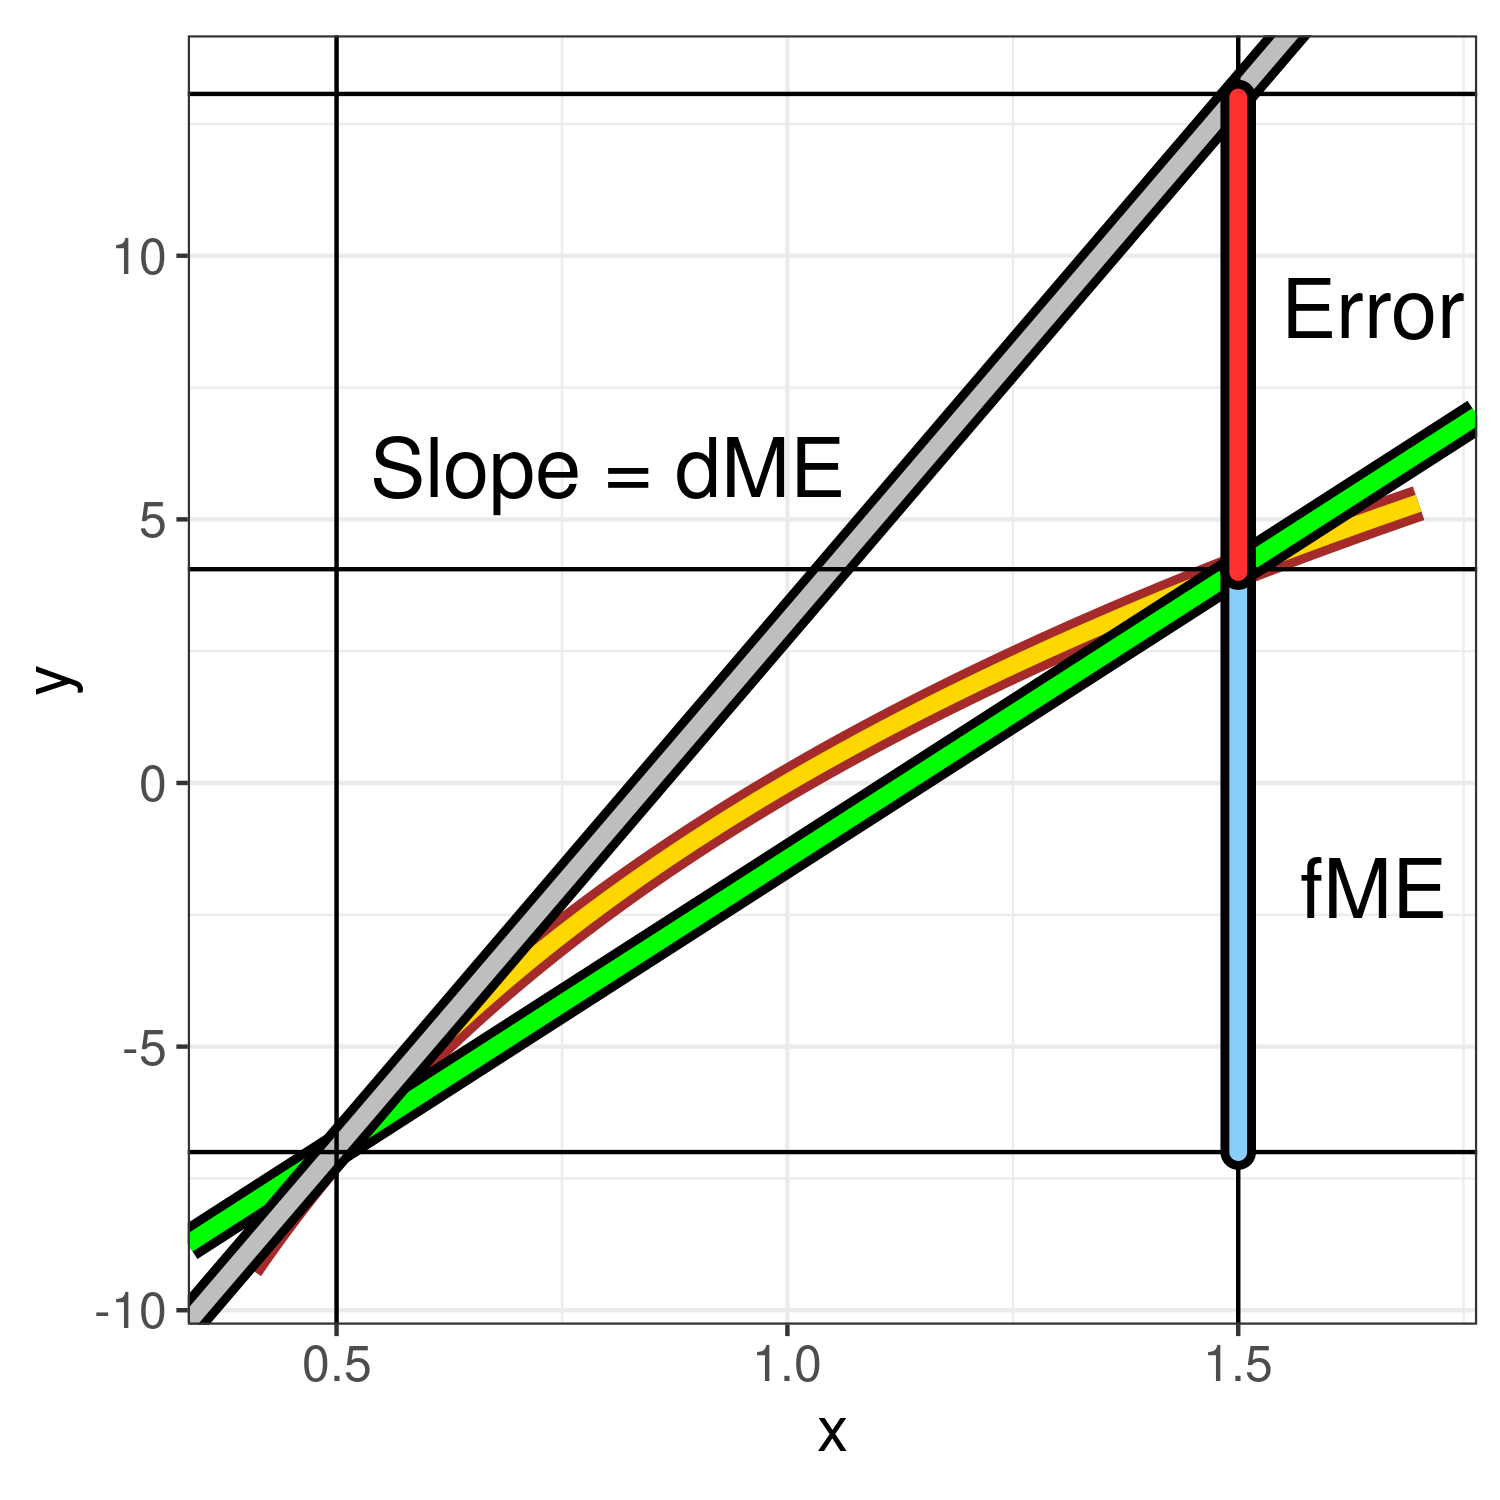
\includegraphics[width=\textwidth]{figure_man/derivative_me_error.png}
% 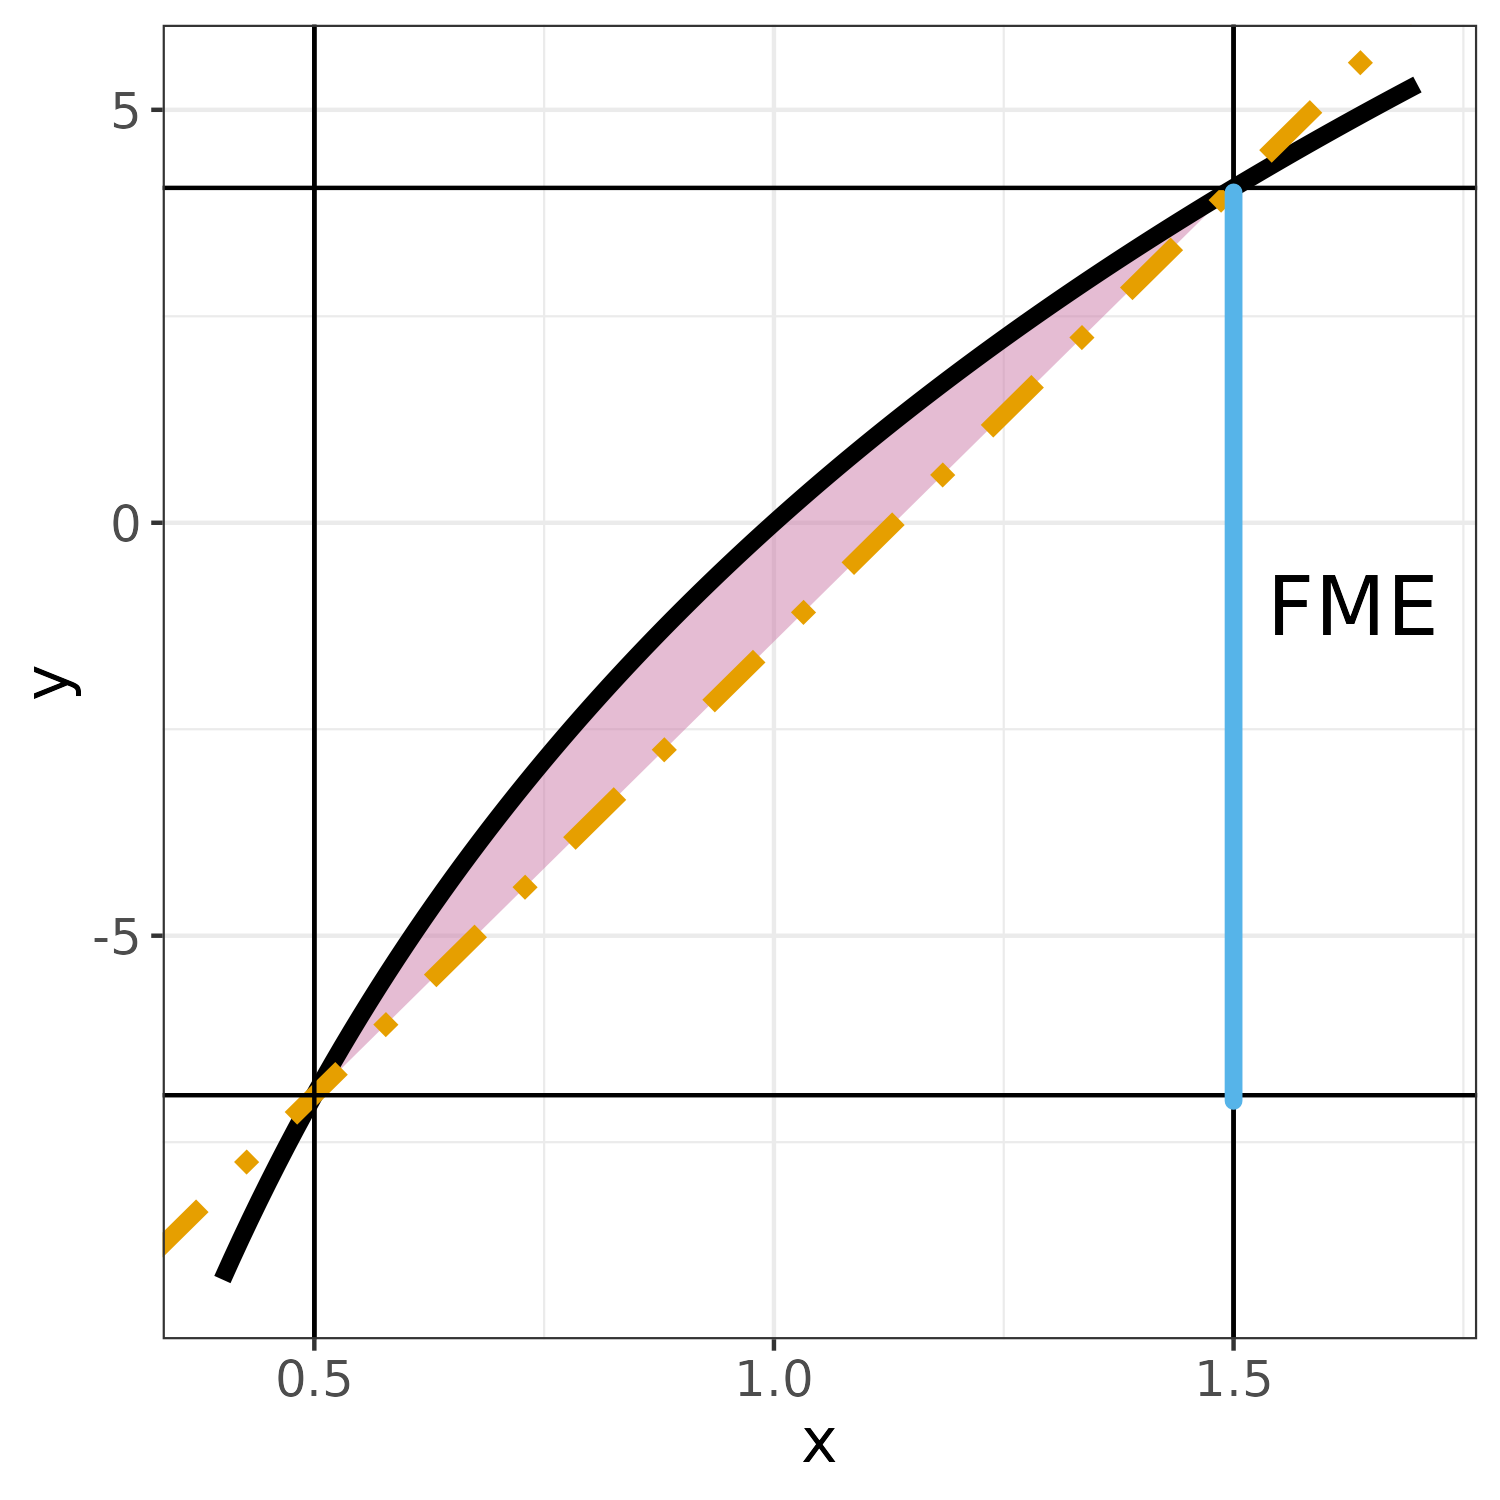
\includegraphics[width=\textwidth]{figure_man/forward_me_deviation.png}
% \end{column}
% \end{columns}
% \end{frame}



% \begin{frame}{Derivative versus Forward Difference}

% %%%

% \begin{columns}[T]
% \begin{column}{0.6\textwidth}
% \begin{itemize}
% \itemsep1em
% \item Derivative of non-linear prediction functions substantially differ at different points \\
% $\Rightarrow$ dME is not suited
% \item fME corresponds to a movement on prediction function, indicating changes in predicted outcome regardless of the function's shape\\
% $\Rightarrow$ fME better suited for non-linear prediction functions
% \item However, with both variants, we lose information about the prediction function along the finite difference
% \end{itemize}
% \end{column}
% \begin{column}{0.4\textwidth}
%  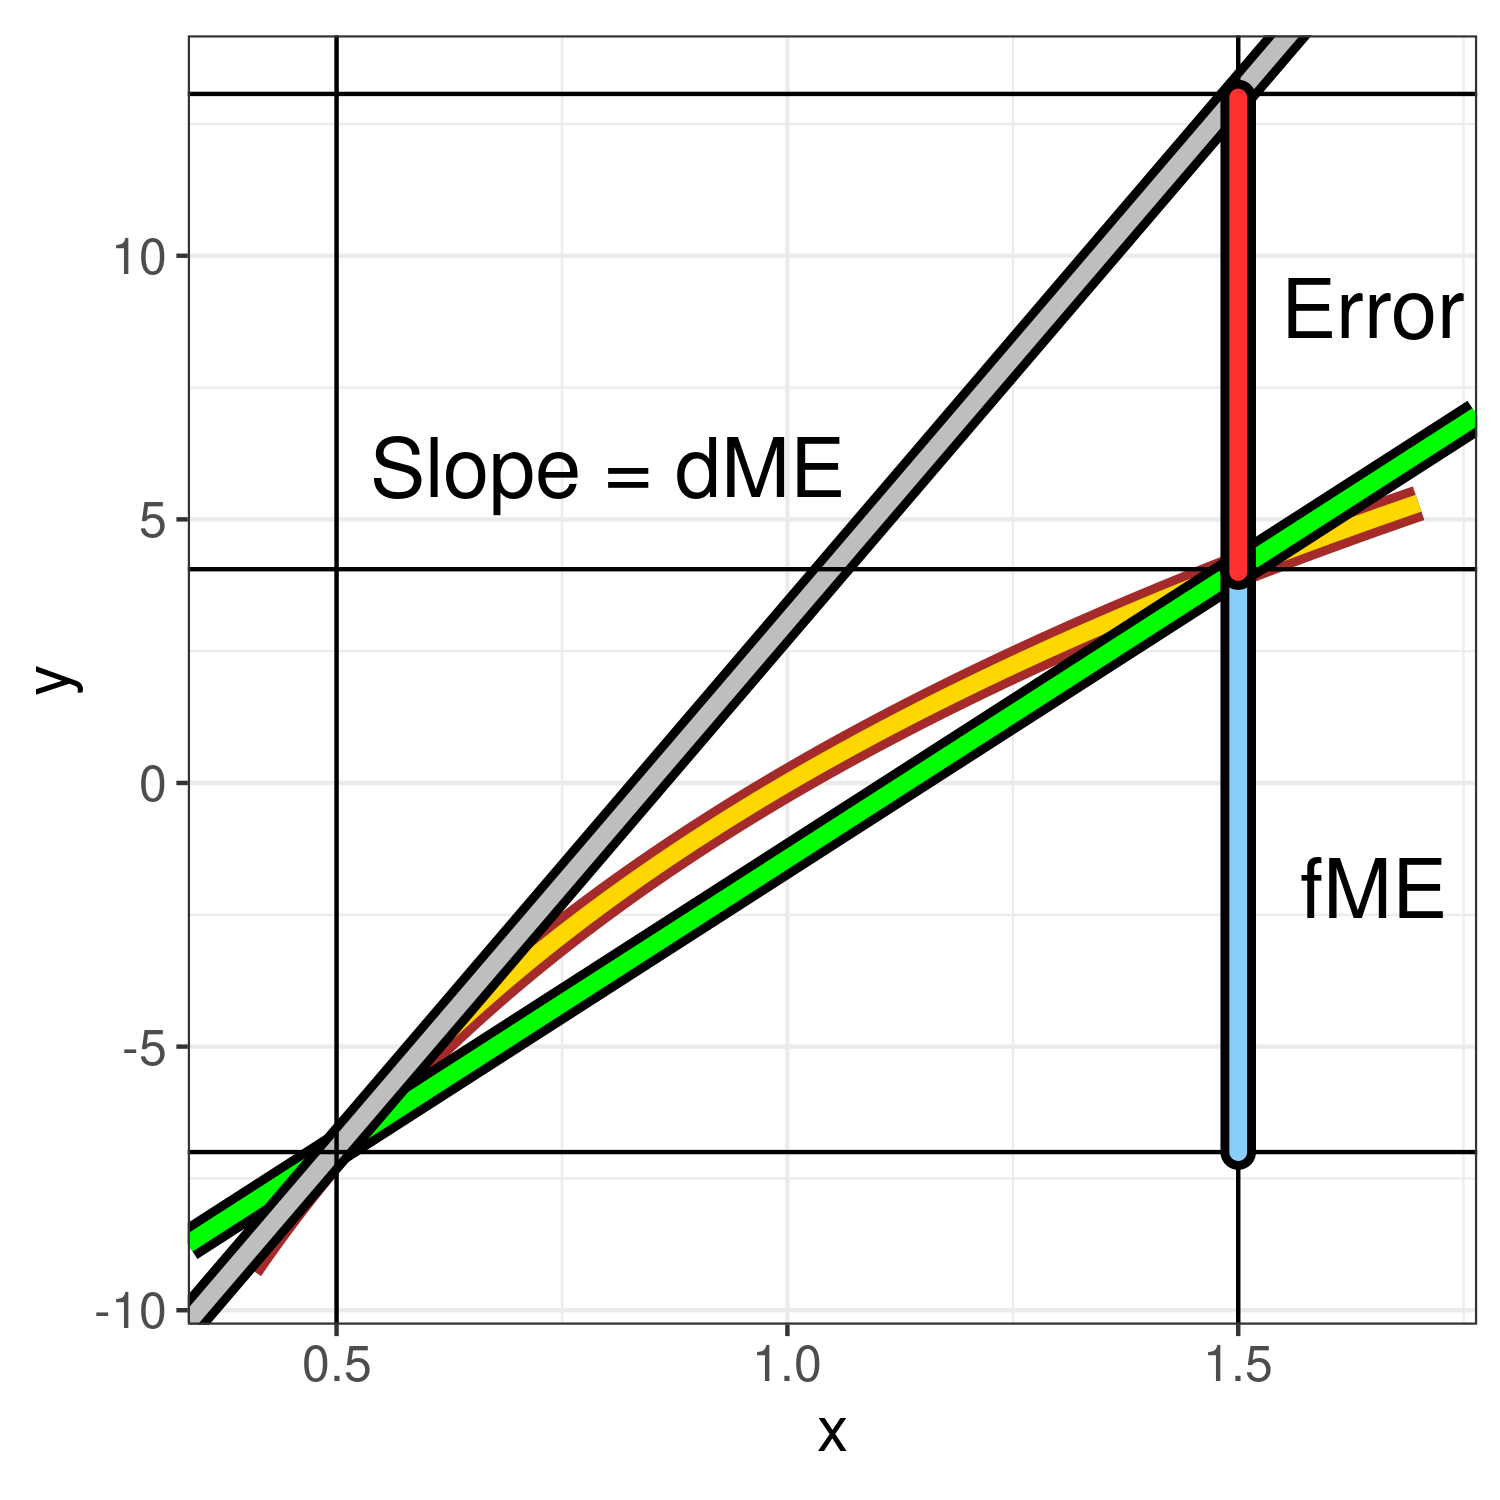
\includegraphics[width = \textwidth]{figure_man/derivative_me_error.png}
% \end{column}
% \end{columns}

% \end{frame}

% \begin{frame}{Derivative versus Forward Difference}
% \begin{figure}
%   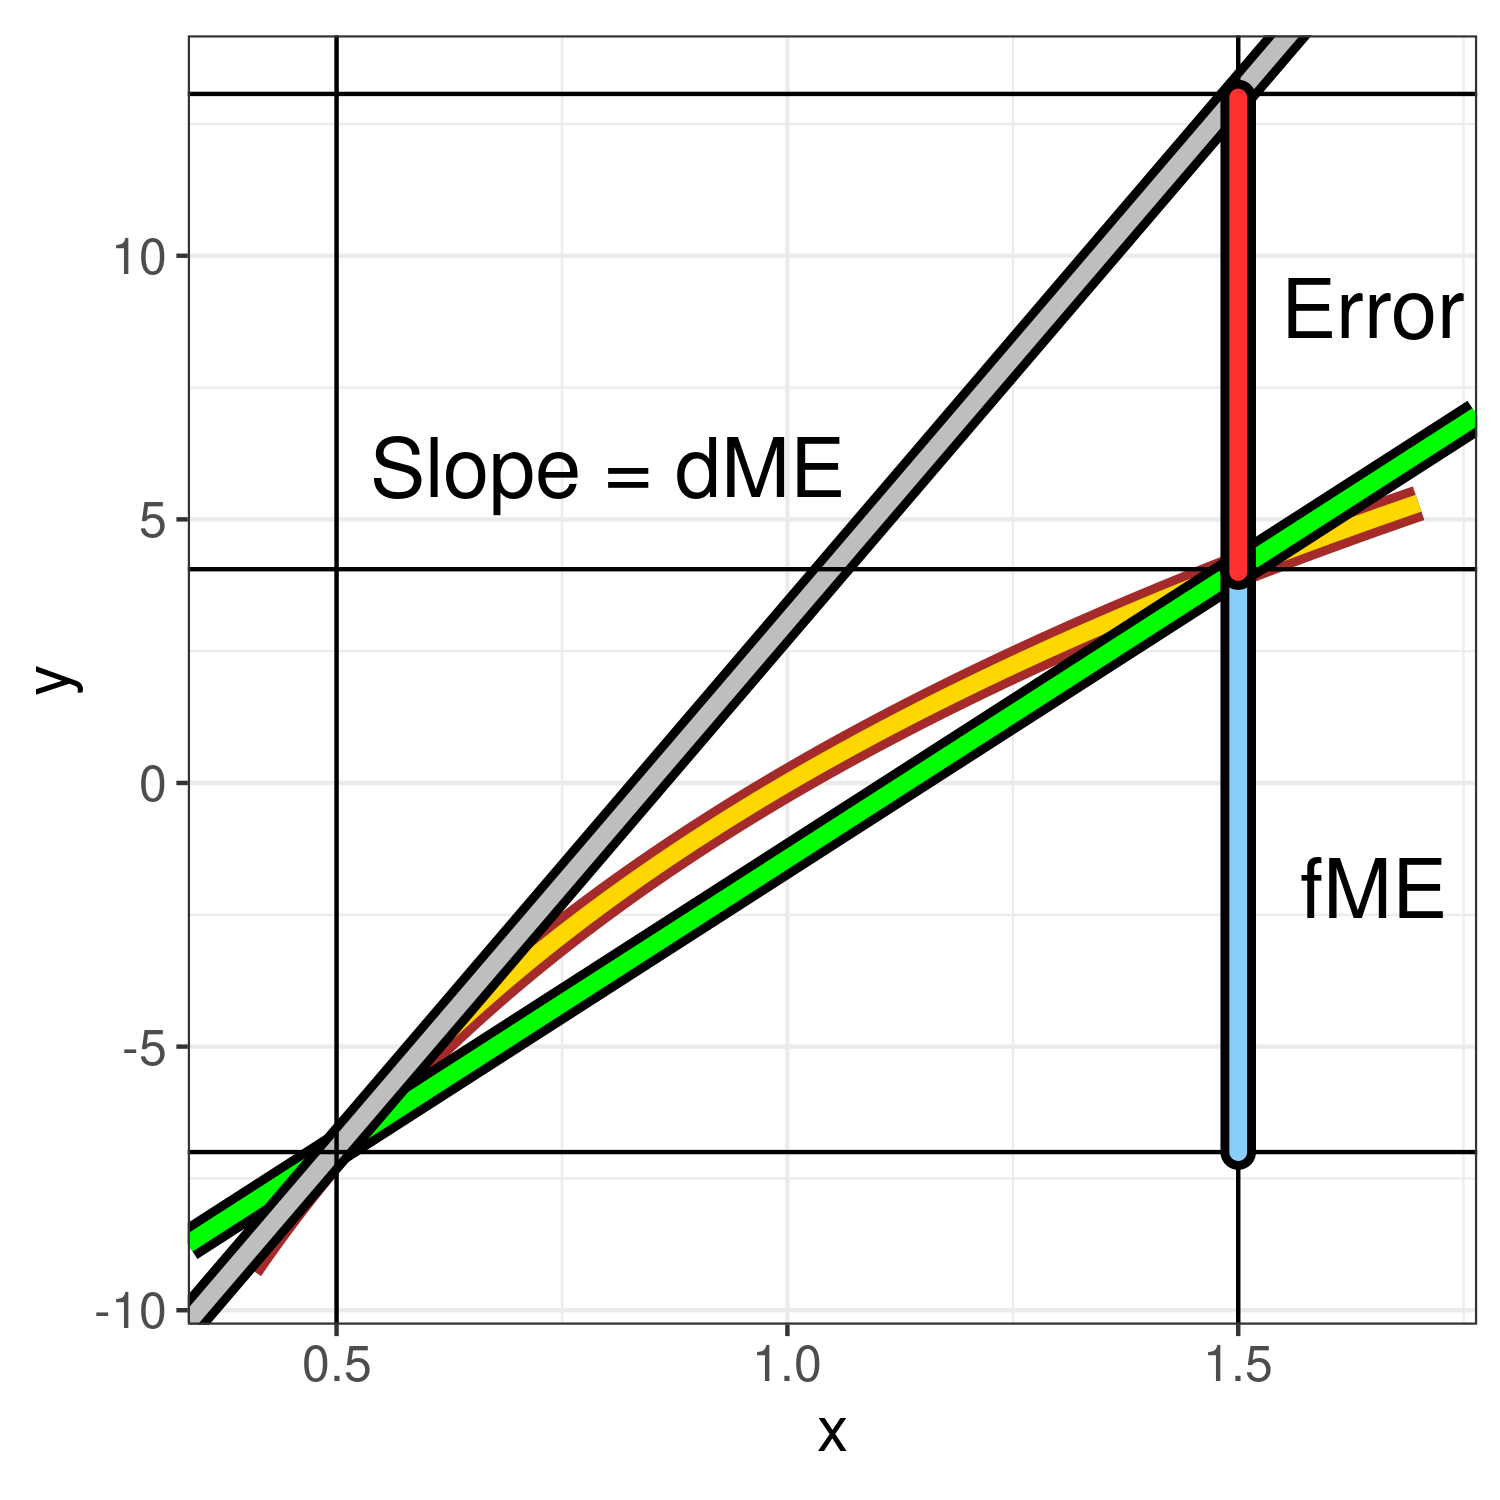
\includegraphics[width = 0.5\textwidth]{figure_man/derivative_me_error.png}
% \end{figure}
% \end{frame}

% ----------------------------------------------------------------
\begin{frame}{Derivative vs.\ Forward Difference}

\begin{columns}[T,onlytextwidth]
% ----- LEFT COLUMN ----------------------------------------------
\begin{column}{0.67\textwidth}
% \begin{itemize}%\setlength\itemsep{0.5em}
  % \item 
  \textbf{dME (tangent, green)}
        \begin{itemize}
            \item slope of the tangent at \(x\);
            \item delivers a \emph{rate} of change \(\tfrac{\partial\widehat f}{\partial x}\).
        \end{itemize}
  % \item 
  \textbf{fME (secant, orange)}
        \begin{itemize}
            \item vertical gap between two model evaluations;
            \item always \emph{exact} change in predicted outcome.
            \item Non-linearity measure (pink band, bottom): quantifies deviation of secant and true curve 
            %We can quantify how much fME secant deviates from the true curve -- a quick "non-linearity measure"’ for each fME (purple band, bottom figure)
        \end{itemize}

  % \item 
  \textbf{When the two differ}
        \begin{itemize}
            \item Curvature makes the tangent overshoot or undershoot  
                  \(\Rightarrow\) dME may be badly biased.
            \item fME is robust to kinks, plateaus, trees, $\dots$
        \end{itemize}
    %\item<2-> Both lead to information loss about prediction function along the finite difference
    % \item
\only<2->{\textbf{Recommendations}}
\begin{itemize}
    \item<2-> Use fME for any non-linear / non-smooth model
    \item<2-> Use dME for lin. func.-s or analytic convenience
\end{itemize}

% \end{itemize}

\end{column}

% ----- RIGHT COLUMN ---------------------------------------------
\begin{column}{0.33\textwidth}
    \centering
    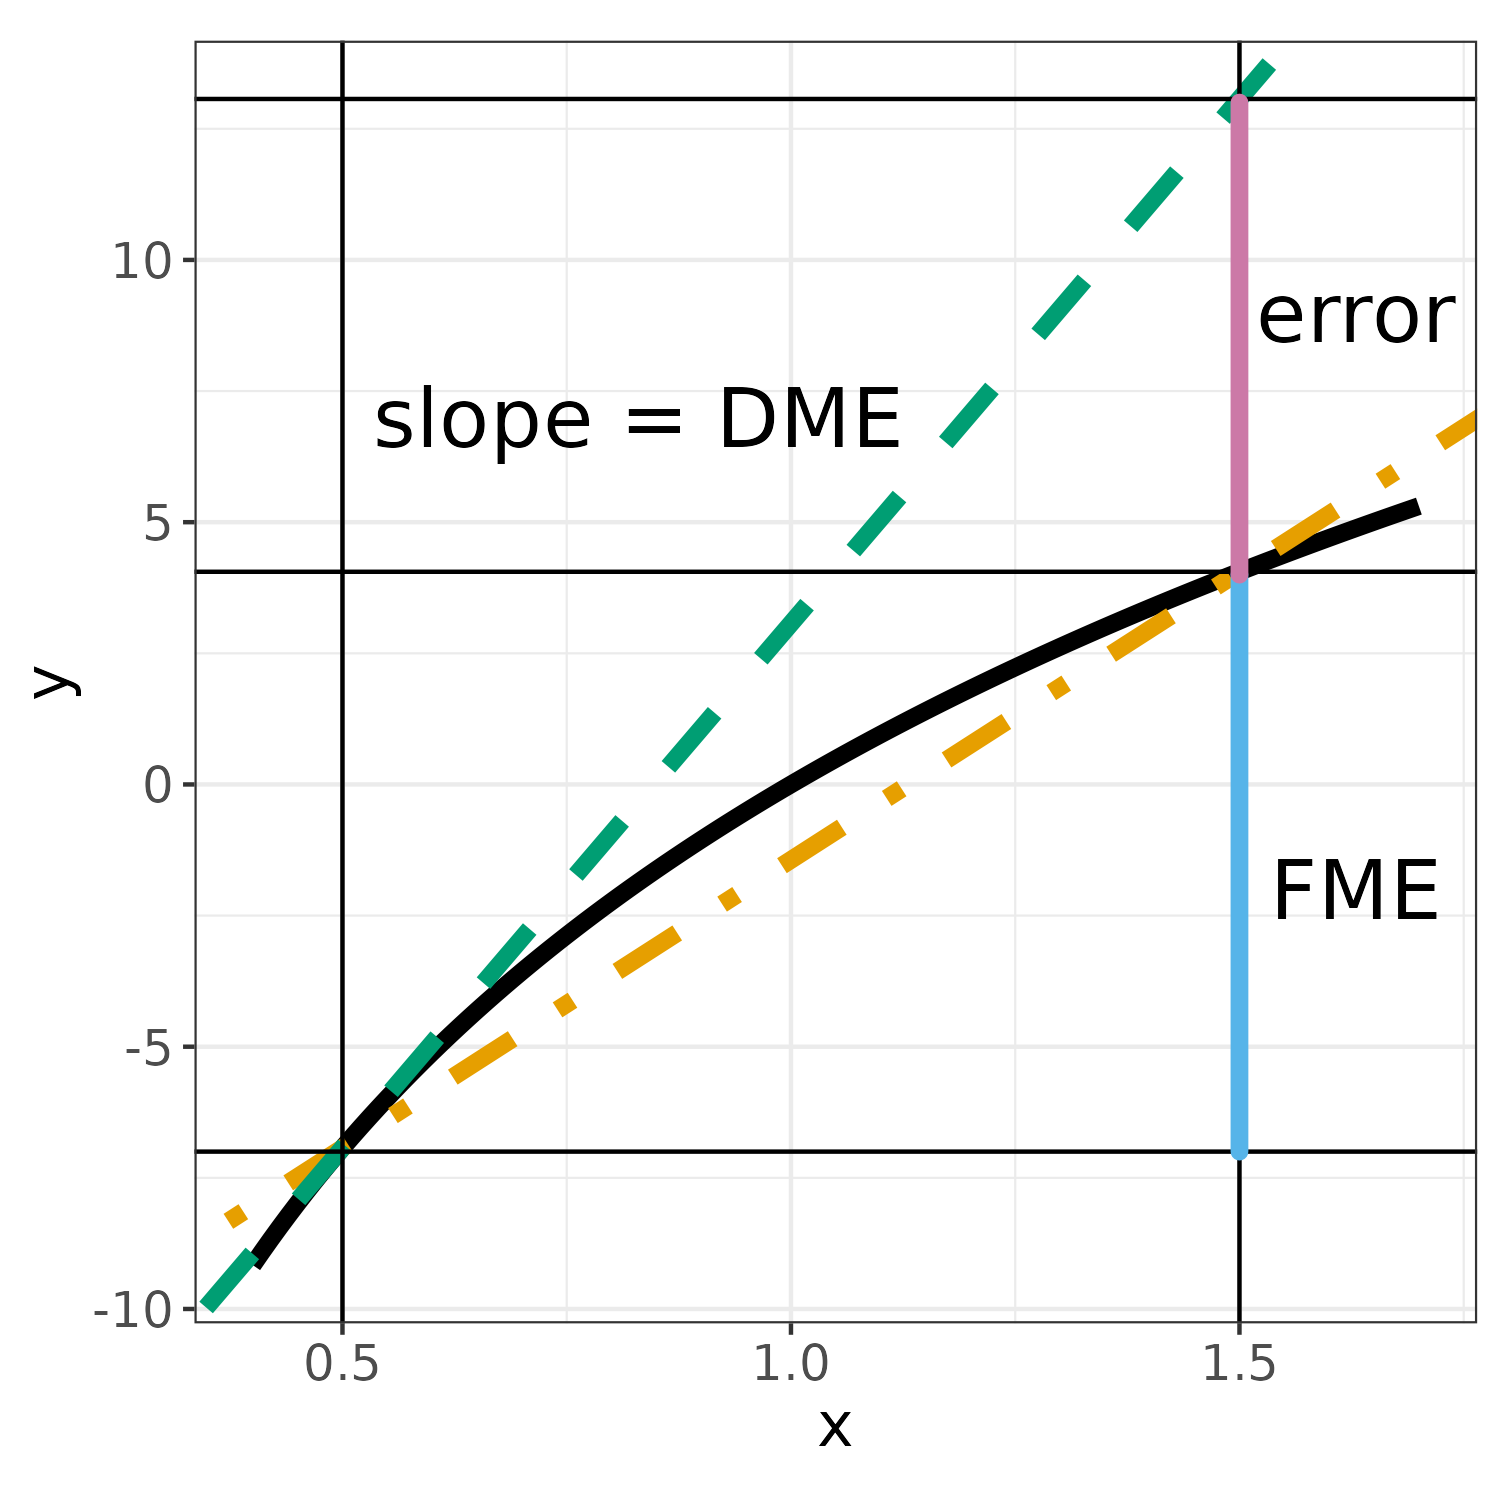
\includegraphics[width=\linewidth]{figure_man/dme_error.png}\\
    \scriptsize
    black = non-lin. function\\
    blue = fME; pink = dME error

    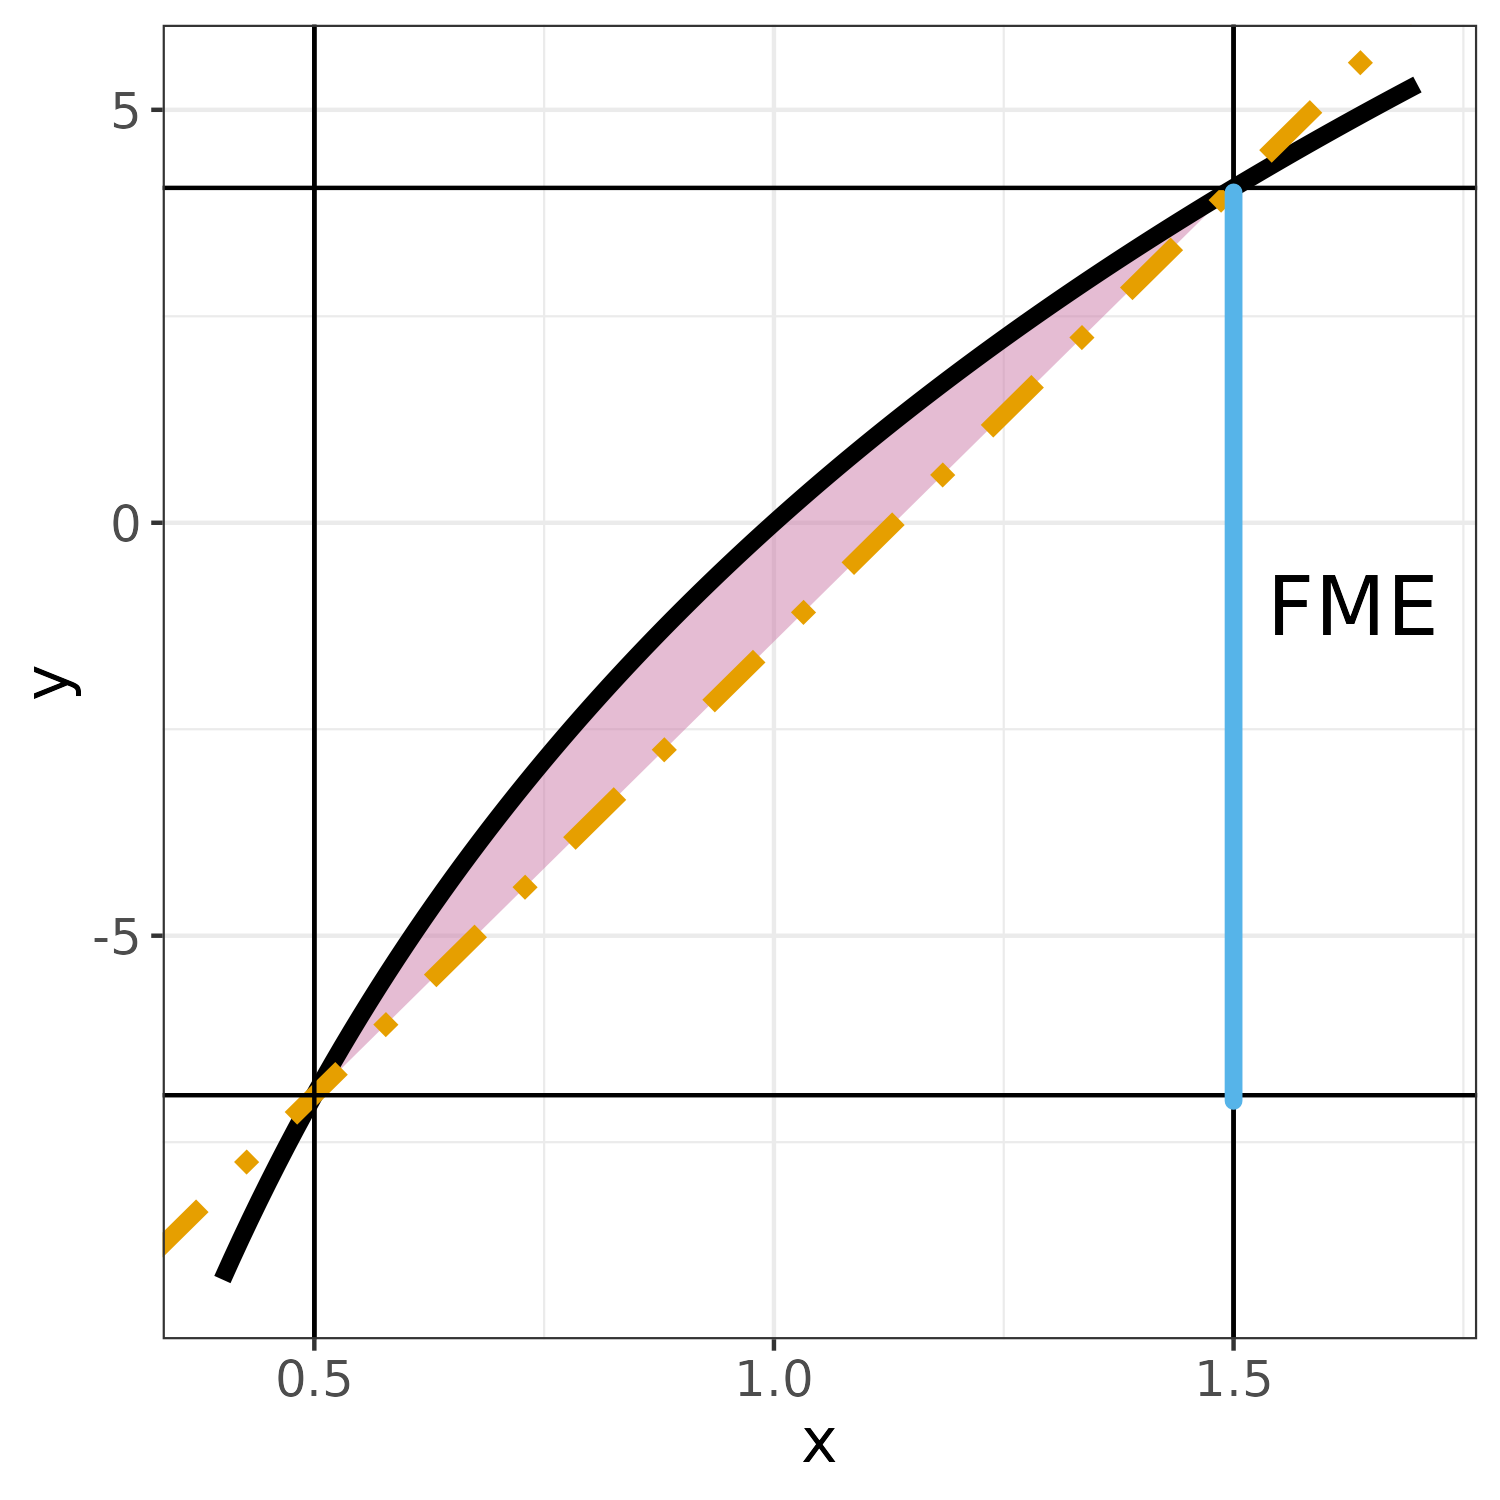
\includegraphics[width=0.8\linewidth]{figure_man/forward_me_deviation.png}
\end{column}
% ---------------------------------------------------------------
\end{columns}
\end{frame}
% ----------------------------------------------------------------


% Marginal Effects for Continuous Features
\begin{frame}{ME for Continuous Features}
\begin{itemize}
\item \textbf{Derivative Marginal Effect (dME)}:
\[
\text{dME}_j(\xv) = \frac{\partial \fh(\xv)}{\partial x_j} \approx \frac{ \fh(x_1, \dots, x_j + h_j, \dots, x_p) -  \fh(x_1, \dots, x_j - h_j, \dots, x_p)}{2h_j}
\]
%where $\mathbf{e}_j$ is the unit vector in the $j$-th direction.
\item \textbf{Forward Marginal Effect (fME)}:
\[
\text{fME}_j(\xv, h_j) = \fh(x_1, \dots, x_j + h_j, \dots, x_p) - \fh(\xv)
\]

% \item \textbf{Example Model}:
% $\fh(\xv)  = \fh(x_1,x_2) = \theta_0 + \theta_{1} x_1^2 + \theta_{2} x_2^2 + \theta_{1,2} x_1 x_2 %+ \epsilon
% $
% \begin{itemize}
% \item Derivative ME of $x_1$:
% \\
% \medskip
% \centerline{$
% \text{dME}_1(\xv) = \frac{\partial \fh(\xv)}{\partial x_1} = 2\theta_1 x_1 + \theta_{1,2} x_2
% $}
% \medskip
% \item Forward ME of $x_1$ with step size $h_1$:
% $$
% \begin{aligned}
% \text{fME}_1(\xv, h_1) 
% &= \fh(x_1 + h_1, x_2) - \fh(x_1, x_2) \\
% &= \theta_1\left((x_1 + h_1)^2 - x_1^2\right) + \theta_{1,2} x_2 h_1 \\
% &= 2\theta_1 x_1 h_1 + \theta_1 h_1^2 + \theta_{1,2} x_2 h_1
% \end{aligned}
% %\theta_1 \left( (x_1 + h_1)^2 - x_1^2 \right) + \theta_{1,2} x_2 h_1 = h_{1}(2\theta_{1}x_{1}+\theta_{1}h_{1}+\theta_{1,2}x_{2})
% $$
% \end{itemize}
\end{itemize}
\begin{itemize}
\item \textbf{Note:} fME is not scale-invariant -- halving the step size does not halve the effect.


\item \textbf{Additive Recovery:} dME and fME isolate terms involving the target feat.
\begin{itemize}
\item \textbf{Example:} For $\widehat{f}(\xv) = a x_1 + b x_2$: 
$\text{dME}_1(\xv) = a$, \quad $\text{fME}_1(\xv, h_1) = a h_1$
\item Effects from additively linked features (e.g., $x_2$) are canceled.
\item Enables focus on direct feature-specific influence in $\widehat{f}$.
\end{itemize}

\end{itemize}

\end{frame}

% % Marginal Effects for Categorical Features
% \begin{frame}{Marginal Effects for Categorical Features}
% \begin{itemize}
% \item \textbf{Traditional Approach}:
% \begin{itemize}
% \item Compute the change in prediction when the feature value changes from a reference category to another category.
% \item For each observation, set the categorical feature to the reference category and record the change in prediction when changing it to every other category.
% \end{itemize}
% \item \textbf{Unified fME Definition for Categorical Features}:
% \[
% \text{fME}_{\xv, c_j} = \fh(c_j, \xv_{-j}) - \fh(x_j, \xv_{-j})
% \]
% \item \textbf{Advantages}:
% \begin{itemize}
% \item Removes ambiguity by treating categorical features similarly to continuous features.
% \item Provides an exact change in prediction for a change in category.
% \end{itemize}
% \end{itemize}
% \end{frame}

% Marginal Effects for Categorical Features
\begin{frame}{ME for Categorical Features}
\begin{itemize}
\item \textbf{Traditional Approach}:
\begin{itemize}
  \item Choose a baseline category for the categorical feature \(x_j\) \\
  $\leadsto$ Either the observed value \(x_j\) or a fixed reference \(x_j^\text{ref}\)
  \item Replace \(x_j\) with an alternative category \(x_j^\text{new}\)
  \item Compute the change in prediction, keeping all other feat. \(\xv_{-j}\) fixed
\end{itemize}
% \begin{itemize}
% \item Estimate the change in prediction when a categorical feature switches from an original $x_j$ or a reference category $x_j^\text{ref}$ to another category $x_j^\text{new}$.
% \item For each observation \(\xv\), hold \(\xv_{-j}\) fixed and vary \(x_j\) across levels.
% %\item For each observation \(\xv\), vary the categorical feature \(x_j\) from a baseline category (either original $x_j$ or \(x_j^\text{ref}\) ) to other levels.
% \end{itemize}
% \item \textbf{Traditional Approach}:
% \begin{itemize}
%   \item Compute prediction differences relative to a fixed reference category \(x_j^{\text{ref}}\).
%   \item For each observation \(\xv\), compare predictions with \(x_j = x_j^{\text{ref}}\) (or using any other baseline category) versus \(x_j = x_j^{\text{new}}\) while holding \(\xv_{-j}\) fixed.
% \end{itemize}

\item \textbf{fME Definition for Categorical Features}:\\
\medskip
\centerline{$
\text{fME}_j(\xv; x_j^\text{new}) = \widehat{f}(x_j^\text{new}, \xv_{-j}) - \widehat{f}(x_j, \xv_{-j})$}
\medskip
\begin{itemize}
\item \(x_j\): original category of feature \(j\) in obs. \(\xv\) (or reference category $x_j^\text{ref}$)
\item \(x_j^\text{new}\): new category to evaluate
\item \(\xv_{-j}\): all other features held fixed
\end{itemize}

\item \textbf{Advantages}:
\begin{itemize}
\item Mirrors continuous feature fME: measures discrete change in pred.
\item Any level can act as baseline - no fixed reference needed.
%Avoids ambiguity from arbitrary reference-category baselines.
\end{itemize}
\end{itemize}
\end{frame}



% \begin{frame}{Additive Recovery}

% \begin{itemize}
% \itemsep1em
% \item Both variants only recover terms within prediction function that depend on feature(s) of interest
% \item Consider a prediction function $\fh(x) = ax_1 + bx_2$. It follows that:
% \begin{align*}
% dME_1(x) &= a \\
% fME_1(x, h_1) &= ah_1
% \end{align*}
% \item MEs remove effects of other features that are linked additively %, regardless of how many remaining features exist, and their effect structure
% \end{itemize}

% \end{frame}


\begin{frame}{Average Marginal Effects}

%\footnotesize

\textbf{Definition (based on fMEs with step $\bm h_S$, can also be based on dMEs)}:
$$\text{AME}_S = \frac{1}{n} \sum_{i=1}^n \big[\fh(\bm x_S^{(i)} + \bm h_S, \bm x_{-S}^{(i)}) - \fh(\bm x^{(i)})\big]$$
%\begin{align*}
%\text{AME}_S &= \frac{1}{n} \sum_{i=1}^n \big[\fh(\bm x_S^{(i)} + \bm h_S, \bm x_{-S}^{(i)}) - \fh(\bm x^{(i)})\big] & \text{Average across all obs. (global summary)}\\
%\text{MEM}_S &= \fh(\bar{\bm x}_S + \bm h_S, \bar{\bm x}_{-S}) - \fh(\bar{\bm x}) & \text{Effect at sample mean (may be unrealistic)}\\
%\text{MER}_S &= \fh(\bm x_S^\ast + \bm h_S, \bm x_{-S}^\ast) - \fh(\bm x^\ast) &  \text{Effect at hand-picked "typical" profile}
%\end{align*}
% \vspace{-0.3em}
% \textbf{Interpretation}:
% \begin{itemize}\setlength\itemsep{0.3em}
% \item \textbf{AME}: Average across all observations (global summary).
% \item \textbf{MEM}: Effect at sample mean (may be unrealistic).
% \item \textbf{MER}: Effect at hand-picked “typical” profile.
% \end{itemize}
\textbf{Why they work in GLMs}:
\begin{itemize}\setlength\itemsep{0.25em}
\item Link function is monotonic $\Rightarrow$ direction of effect stable.
\item Averaging gives sensible results (e.g., logit, probit).
\end{itemize}

\vspace{0.2em}
\textbf{Why they fail on non-parametric models}:
\begin{itemize}%\setlength\itemsep{0.25em}
\item AMEs assume a consistent effect across the feature space.
\item Non-parametric models can model complex, non-linear relationships.
\item Averaging effects can obscure important heterogeneities.
\end{itemize}
%\item Non-linear $\fh$ may flip sign, saturate, or interact \\$\Rightarrow$ AME $\approx$ 0 despite strong local effects.
%\item MEM may use invalid input (e.g., "mean gender").
%\item MER depends on arbitrary choice of profile.
%\item \textbf{Takeaway:} Use \textbf{cAMEs}, \textbf{LLTRs}, and \textbf{NLMs} to respect heterogeneity.
%\end{itemize}

\vspace{0.2em}
\textbf{Takeaway:} AMEs can be useful summaries for smooth, monotonic models.  
For black-boxes, use \textbf{local fMEs} and support them with non-linearity measure.

\end{frame}


% % Additive Recovery Property
% \begin{frame}{Additive Recovery Property}
% \begin{itemize}
% \item Both dME and fME recover only terms involving the feature(s) of interest.
% \item \textbf{Example}:
% \[
% \widehat{f}(\xv) = a x_1 + b x_2
% \]
% Then:
% \begin{align*}
% \text{dME}_1(\xv) &= a \\
% \text{fME}_1(\xv, h_1) &= a h_1
% \end{align*}
% \item Effects of other features linked additively are removed.
% \item This property allows focusing on the direct effect of the feature.
% \end{itemize}
% \end{frame}

















% \begin{frame}{Marginal Effects}

% \begin{itemize}
% %\itemsep2em
% \item
% Derivative ME: Derivative of $f$ w.r.t. feature. Compute via numeric differentiation
% $$dME_j(x) = \frac{\partial f(x)}{\partial x_j} \approx \frac{f(x + h) - f(x - h)}{2h}$$
% \item Less known definition based on forward differences: Change in predicted outcome due to a change in feature value (e.g., increasing a feature $x_j$ by $h_j$) $\Rightarrow$ forward ME (fME):
% \begin{equation*}
% fME_j(x, h_j) = f(x_1, \dots, x_j + h_j, \dots, x_p) - f(x)
% \end{equation*}
% \item Example: For model equation $y = \theta_0 + \theta_{1} x_1^2 + \theta_{2} x_2^2 + \theta_{1, 2} x_1 \cdot x_2 + \epsilon$
% \begin{itemize}
% \item dME of $x_1$ is $dME_1(x) = 2\theta_1 x_1 +  \theta_{1, 2} x_2$
% \item fME of $x_1$ with step size $h_1 = 1$ is
% $fME_1(x, h_1) = 2\theta_1 h_1^2 +  \theta_{1, 2} x_2 h_1$
% \end{itemize}
% \end{itemize}
% \end{frame}


%%%
%------------------------------------------------------------
% \begin{frame}{Why Marginal Effects \emph{still} matter}
% \begin{itemize}
%   \item \textbf{Scalar answers}: fME/AME $=$ $\Delta\hat y$ per $\Delta x$ - easy to quote, store, regress on.  
%   \item \textbf{High-dimensional moves}: change several features at once\\
%   $\leadsto$ PD/ICE plots collapse beyond 2-D
%   \item \textbf{Categoricals included}: fME\(c_j\) = $\hat f(\text{new cat})-\hat f(\text{old})$ - no dummy coding.  
%   %\item \textbf{No feature-independence assumption}: we perturb the \emph{observed} point – avoids unrealistic combos that PD may sample.
%   % \item \textbf{Local trust score}: NLM \(\uparrow\) tells when the linear view holds (LLTR), something PD/ICE can’t quantify numerically.  
%   % \item \textbf{Statistical workhorses}: averages (AME/cAME), CIs, hypothesis tests, subgroup trees – all built on numeric MEs.  
%   \item \textbf{Efficiency}: two predictions per observation vs.\ grid\(\times n\) evaluations for PD.  
% \end{itemize}
% %\vspace{0.2cm}
% %\alert{Plots help you \emph{see}; Marginal Effects give numbers you can \emph{use}.}


% \begin{block}{Key points}
% \begin{enumerate}[1.]
% \item \textbf{PD / ICE} excel at \alert{exploration and storytelling}:  you \emph{see} how predictions evolve.
% \item \textbf{Forward Marginal Effects} deliver \alert{concise, numeric,
%       statistically-tractable} answers that
%       regulators, tables, and downstream pipelines need:
%       \begin{itemize}
%           \item single numbers (AME, cAME) with CIs;
%           \item high-dimensional interventions possible;
%           \item no independence assumption, no surrogate model.
%       \end{itemize}
% \end{enumerate}
% \end{block}

% \begin{center}
% \Large\(\Rightarrow\) \textbf{Use both: plots to explore, MEs to quantify.}
% \end{center}
% \end{frame}
% --------------------------------------------------------------- %
%  Slide – Why Marginal Effects still matter (Concise, Formal)
% --------------------------------------------------------------- %
% \begin{frame}{Why Marginal Effects \emph{still} matter}

% \begin{itemize}\setlength\itemsep{0.4em}
%   \item \textbf{Scalar summary:}  
%         $\text{fME}$ are easy to quote, store, regress on.

%   \item \textbf{High-dimensional changes}: change several features at once (incl. categorical)\\
%   $\leadsto$ Avoids dimensionality constraints from visualizations (PD/ICE)
        
%   \item \textbf{Model-faithful:}  
%         Local to $\xv$; preserves interactions without assumptions.
%    \item \textbf{Non-Linearity Measure (NLM)}: Complements ME values by quantifying how well a local linear approximation holds. High NLM value indicates that ME is locally reliable - something PD/ICE plots cannot quantify. 
%   \item \textbf{Efficient:}  
%         Two predictions per feature suffice.
%   \item \textbf{Conclusion:}
%   \begin{itemize}
%       \item ME yield concise, rigorous insights
%       \item Complementary to PD/ICE visualizations
%   \end{itemize}
% \end{itemize}

% \end{frame}

% ---------------------------------------------------------------- %
%  Slide – Why Marginal Effects still matter
% ---------------------------------------------------------------- %
\begin{frame}{Why Marginal Effects \emph{still} matter}

\begin{itemize}\setlength\itemsep{0.55em}
% ----------------------------------------------------------------
\item \textbf{Single, formal number:} One \alert{scalar} per observation; can be averaged (AME), reported with CIs, audited, stored easily.

% ----------------------------------------------------------------
\item \textbf{Multivariate changes}  
      Simultaneously perturb multiple \emph{continuous/categ.} feat.
       Still yields a scalar (unlike PD/ICE, which require multivar. plots).
      %No dimensionality issues from visualizations (PD/ICE).

% ----------------------------------------------------------------
\item \textbf{Model-faithful, assumption-light}  
      Measured at the \emph{actual data point}.
      Captures interactions, no indep. or surrogate-model assumptions (LIME).

% ----------------------------------------------------------------
\item \textbf{Non-Linearity Measure:}  
Quantifies how well local linear approximation holds (e.g., via a normalized squared deviation from the secant). \\
$\leadsto$ Local reliability measure, something PD/ICE plots cannot quantify.
% ----------------------------------------------------------------
\item \textbf{Computationally cheap}  
      Just two forward passes (or \(k\!-\!1\) for a \(k\)-level factor) per observation vs.\ grid\(\times n\) for PD/ICE.

\end{itemize}

\vspace{0.3em}
\textbf{Conclusion:} 
\begin{center}
\textbf{Plots let you \emph{see} the landscape;\quad  
ME give numbers you can \emph{use}.}
\end{center}

\end{frame}

% --------------------------------------------------------------- %
%  Slide – Clinician use-case: Marginal Effects vs ICE/PD
% --------------------------------------------------------------- %
\begin{frame}{Use-case: Scalar vs. Visual Estimation}

\textbf{Setting:}  
A clinical model predicts heart attack risk from patient features, e.g., $x_1:$ systolic blood pressure (BP), $x_2:$ LDL cholesterol, $x_3:$ age, ...

\vspace{0.5em}
\textbf{Clinician’s questions}
\begin{itemize}\setlength\itemsep{0.3em}
  \item \emph{"What if this patient’s systolic BP increases by 10 mmHg?"}
  \item \emph{"What if BP increases by 10 mmHg \& LDL by 15 mg/dL?"}
\end{itemize}

\vspace{0.5em}
\textbf{Route A – ICE / PD}
\begin{itemize}
  \item Plot prediction as a function of BP (1-D) or BP+LDL (2-D) on a grid.
  %Visualize effect along 1-D or 2-D feature grid.
  \item Manual interpretation of change by looking at curve/surface.
  \item[\(\rightarrow\)] Visual and local; limited to 1–2 features at a time.
\end{itemize}

\vspace{0.3em}
\textbf{Route B – Forward Marginal Effect}: $\mathrm{fME}
  = \widehat f(\xv + \mathbf{h}) - \widehat f(\xv)$
\begin{itemize}
  \item \textbf{1-D case:} \(\mathbf{h} = (10, 0, 0, \dots) \;\Rightarrow\;\) risk increases by \textbf{+3 \% points}
  \item \textbf{2-D case:} \(\mathbf{h} = (10, 15, 0, \dots) \;\Rightarrow\;\) risk increases by \textbf{+4.1 \% points}
  \item One scalar answer per query, extensible to higher dimensions.
\end{itemize}

\end{frame}

% % ---------------------------------------------------------------- %
% %  Slide 1 – Clinician use-case: two interpretation routes
% % ---------------------------------------------------------------- %
% \begin{frame}{Use-case}

% \textbf{Clinician’s question}  
% \emph{"If this patient’s systolic blood pressure rises by 10 mmHg,
% how will her predicted heart-attack risk change?"}

% \vspace{0.6em}
% \begin{columns}[t,onlytextwidth]

% % ---------- left column: ICE / PD vs fME ------------------------ %
% \begin{column}{1\textwidth}
% \textbf{Route A – ICE / PD}  
% \begin{itemize}
%   \item Draw ICE curve for the patient across BP grid.
%   \item Read the distance between 120 and 130 mmHg.  
%         \(\rightarrow\) visual, manual, 1-D only.
% \end{itemize}

% \medskip
% \textbf{Route B – Forward Marginal Effect}  (\(h=10\))
% \[
% \mathrm{fME}_{\Delta\text{BP}=10}
%   \;=\; \widehat f(\text{BP}+10,\xv_{-\text{BP}})
%   -   \widehat f(\xv)
%   \;=\; \mathbf{+3\;\text{pp}}
% \]
% \begin{itemize}
%   \item One scalar answer: "+3 percentage-points risk".
%   \item Same formula works for any multi-feature change.
% \end{itemize}
% \end{column}

% % ---------- right column: space for figure if desired ------------ %
% % \begin{column}{0.42\textwidth}
% % \begin{center}
% % %\includegraphics[width=\linewidth]{figure_man/bp_ice_vs_fme_placeholder} % optional
% % \end{center}
% % \end{column}

% \end{columns}
% \end{frame}

% \begin{frame}{Use-case}

% \textbf{Clinician’s question}  
% \emph{"If this patient’s systolic blood pressure rises by 10 mmHg, and LDL cholesterol increases by 15 mg/dL, how will her predicted heart-attack risk change?"}

% \vspace{0.6em}
% \begin{columns}[t,onlytextwidth]

% \begin{column}{1\textwidth}
% \textbf{Route A – ICE / PD}  
% \begin{itemize}
%   \item Examine ICE curves for BP and LDL separately.
%   \item Joint effect estimation requires visual extrapolation.
%   \item \(\rightarrow\) limited to pairwise views, ignores interaction.
% \end{itemize}

% \medskip
% \textbf{Route B – Forward Marginal Effect}  (\(h = (\Delta\text{BP}, \Delta\text{LDL})\))
% \[
% \mathrm{fME}_{\Delta\xv}
%   = \widehat f(\xv + h) - \widehat f(\xv)
%   = \mathbf{+4.1\;\text{pp}}
% \]
% \begin{itemize}
%   \item One scalar for the combined directional effect.
%   \item Automatically incorporates nonlinear interactions.
% \end{itemize}
% \end{column}

% \end{columns}
% \end{frame}


% Relation to ICE and PD
\begin{frame}{Relation to ICE and PD}
\begin{itemize}
\item \textbf{Individual Conditional Expectation (ICE)}:
\begin{itemize}
\item Visualizes predictions for an obs. across a range of feature values.
\item fME corresponds to vertical diff. between points on an ICE curve.
\end{itemize}
\item \textbf{Partial Dependence (PD)}:
\begin{itemize}
\item Shows average predictions across a range of feature values.
\item AME is equivalent to vertical differences on PD for linear models.
\end{itemize}
\item \textbf{Advantages of fMEs}:
\begin{itemize}
\item Provide exact change in prediction.
\item Applicable to high-dimensional feature changes.
\item Quantifiable and not limited to visual interpretation.
\end{itemize}
\end{itemize}
\end{frame}




% \begin{frame}{Model-Agnostic Applicability}

% \begin{itemize}
% \itemsep1em
% \item MEs were historically used to interpret GLMs, however, they can be used as model-agnostic interpretation tools for non-parametric models 
% %\item As fMEs are better suited for non-linear prediction functions, they are better suited for interpreting ML models
% \item fMEs correspond to an exploration of the prediction function and are better suited for non-linear prediction functions
% \item With fMEs, we can also use multivariate changes in feature values to explore the prediction surface in various directions simultaneously
% \item Note: Shape of the prediction function may vary considerably along the forward difference, i.e., an fME with half the step size may not result in half the fME
% \end{itemize}

% \end{frame}


% \begin{frame}{Model-Agnostic Applicability}

% \begin{itemize}
% \itemsep2em
% \item MEs are traditionally used to interpret parametric models such as GLMs. However, both dME and fME can be used as model-agnostic interpretation tools for non-parametric models. As the fME is better suited for non-linear prediction functions, it is the natural choice for black box ML models.
% \item The fME essentially correspond to an exploration of the prediction function. We can also use multivariate changes in feature values to explore the prediction surface in various directions simultaneously.
% \item One needs to keep in mind that the shape of the prediction function may vary considerably along the forward difference, i.e., an fME with half the step size may not result in half the fME.
% \end{itemize}

% \end{frame}





\endlecture
\end{document}
